\documentclass[11pt]{article}
\usepackage[margin=1in]{geometry}
\usepackage[T1]{fontenc}
\usepackage{lmodern}
\usepackage{amsmath,amssymb,booktabs,graphicx,array,tabularx}
\usepackage{icomma} % 16,671 in math mode: no space after a thousands comma
\usepackage[round]{natbib}
\usepackage{placeins}
\usepackage{underscore} % refs.bib notes contain file names with underscores
\usepackage{xurl}
\usepackage[hidelinks]{hyperref}

% Result numbers and process facts. Generated by `crew.py numbers`; never typed by hand.
% Generated by `crew.py numbers` from claims.jsonl. Do not edit by hand.
% Each macro is a number taken from a logged run; see claims.jsonl.

% Generated by `crew.py numbers` from reviews/, runs/ and replication.json. Do not edit by hand.
% Use these macros for any statement about how the paper was made (rounds, runs, rerun).
\newcommand{\CrewReviewRounds}{14}  % review records in reviews/
\newcommand{\CrewRoundsQuestion}{4}  % rounds of the question review
\newcommand{\CrewRoundsLiterature}{2}  % rounds of the literature review
\newcommand{\CrewRoundsDesign}{4}  % rounds of the design review
\newcommand{\CrewRoundsCode}{3}  % rounds of the code review
\newcommand{\CrewRoundsResults}{1}  % rounds of the results review
\newcommand{\CrewRoundsPaper}{0}  % rounds of the paper review
\newcommand{\CrewFindingsCritical}{3}  % distinct critical findings raised (a finding carried across rounds counts once, at its latest severity)
\newcommand{\CrewFindingsMajor}{15}  % distinct major findings raised (a finding carried across rounds counts once, at its latest severity)
\newcommand{\CrewFindingsMinor}{37}  % distinct minor findings raised (a finding carried across rounds counts once, at its latest severity)
\newcommand{\CrewReviewerModels}{claude-opus-5-5}  % models the Reviewer ran on
\newcommand{\CrewReviewIndependence}{fresh-context}  % how independent the reviews were
\newcommand{\CrewRuns}{26}  % runs in the ledger
\newcommand{\CrewRunsAnalysis}{20}  % analysis runs
\newcommand{\CrewRunsDataPrep}{6}  % data-prep runs
\newcommand{\CrewRunsSuperseded}{2}  % runs replaced by a later run with the same id (archived)
\newcommand{\CrewRunsUnreviewed}{0}  % analysis runs not covered by a passing code review
\newcommand{\CrewResultClaims}{974}  % result claims
\newcommand{\CrewCitationClaims}{51}  % citation claims
\newcommand{\CrewRerunReproduced}{0}  % runs the clean rerun reproduced
\newcommand{\CrewRerunTotal}{0}  % runs the clean rerun re-executed
\newcommand{\CrewRerunStatus}{not run}  % outcome of the latest clean rerun


\setlength{\emergencystretch}{2em}
\renewcommand{\topfraction}{0.9}
\renewcommand{\bottomfraction}{0.8}
\renewcommand{\textfraction}{0.07}
\renewcommand{\floatpagefraction}{0.8}

\newcommand{\Q}[2]{#1Q#2}            % calendar quarter, e.g. \Q{2023}{3}
\newcommand{\SEs}{\mathrm{SE}_{s}}
\newcommand{\SEn}{\mathrm{SE}_{n}}
\newcommand{\cand}[1]{\texttt{#1}}   % candidate and run identifiers

\title{A Pre-Specified Update on California's\\ \$20 Fast-Food Minimum Wage: Inconclusive Employment\\
Effects in Limited-Service Restaurants, 2024Q2--2026Q1}
\author{Bryce Wang (human PI) \\ \small Drafted with Free-Research-Crew; see the AI-use statement.}
\date{\today}

\begin{document}
\maketitle

% Abstract. Written last; every claim is checked against Sections 6 and 7 and is no stronger.
% Claims: r-v-h2-headline, r-h2-emp-h2-att/lo95/hi95, r-v-h2 (label probabilities),
% r-v-s1, r-v-s2, r-sec-cemn-s1-att, r-sec-dube-s2-att, r-v-h1, r-h1-wage-h1-att/t/c-hi95,
% r-tnu-h1-95, r-ph-h1-joint, r-v-h3, r-plc-nonff-sign.
\begin{abstract}
California's AB 1228 set a \$20 minimum wage for workers at large fast-food chains from April
2024, and the published QCEW-based estimates of its employment effect disagree. We report a
pre-specified, not blind, update for private limited-service restaurants (NAICS 722513) in
2024Q2--2026Q1, a window that adds the preliminary 2026Q1. A rule fixed before any post-period
outcome was computed picked the primary estimator from 24 candidates on data through 2019: a
trend-adjusted difference in differences with population-weighted donors from all other states.
Inference is built for one treated state. The pooled effect on log employment is $\HTwoAtt$
(95\% interval $\HTwoLoNinetyFive$ to $\HTwoHiNinetyFive$). The pre-specified label is
``inconclusive'', and it is qualified as not separable from a California-wide shock, because
employment outside 722513 also ran above its counterfactual. The design could not have shown an
effect smaller than 2\%: before any post-period data were read, the power run gave that label
probability $\ProbTauZeroUndSmaller$ even with no effect, so the result does not discriminate
between the published estimates. Re-estimations of both published approaches are also
inconclusive ($\SOneAtt$ and $\STwoAtt$). The weekly-earnings first stage, $\HOneAtt$ log
points, is not supported at the pre-specified critical value ($t = \HOneT$ against $\HOneCrit$),
which is not evidence that earnings did not rise; by the design's rule the employment estimate is
then uninformative about the wage floor. Two post hoc checks of that
verdict point in opposite directions. The year-two comparison is uninformative by rule.
\end{abstract}


% Introduction. Written after the results gate from the result claims; every number is a macro.
% Claims: r-sel-candidate, r-v-h2-headline, r-h2-emp-*, r-v-h2 (label probabilities), r-h90-h2,
% r-mde-h2, r-plc-nonff-sign, r-v-s1, r-v-s2, r-v-h1, r-h1-wage-*, r-v-h2-note, r-ph-h1-joint,
% r-v-h3, r-v-n-not-robust.
\section{Introduction}
\label{sec:intro}

On April 1, 2024 California raised the minimum wage of workers at fast-food chains with at least
60 establishments nationwide to \$20 an hour, under Assembly Bill 1228. The studies that
estimate its effect on employment from the same administrative data, the Quarterly Census of Employment and Wages
(QCEW), disagree. \citet{clemens2026employment} find that California's fast-food employment fell
by about 3.5 percent relative to the rest of the country over two years; \citet{dube2026labor}
finds an effect near zero with a different comparison group, outcome normalisation and
estimator. The disagreement has been decomposed into these choices
\citep{dube2026labor,clemens2026synthetic,sosinskiy2026effects}, which means that anyone who
re-estimates the effect knows in advance which choices give which answer.

We ask whether AB 1228 changed employment in California's private limited-service restaurants
(NAICS 722513) over its first eight quarters, 2024Q2--2026Q1, relative to the same industry in
other states, and whether the effect changed between the first and the second year, when the
law's premium over California's general minimum wage fell. Because the specification choices
and their published consequences were known, we did not choose a specification. Before any
outcome after 2023Q3 was computed we fixed the estimand, the base quarter, decision rules for
every label, an inference procedure built for one treated state, and a rule that picks the
primary estimator from 24 candidates covering both published approaches by how well each
reproduced California's own path at placebo dates in 2016--2017, using only data through 2019.
Both published approaches are also re-estimated as named secondary analyses. The study is
pre-specified but not blind: its authors knew the published estimates and a public descriptive
series through March 2026 before the design was fixed (Section~\ref{sec:prespec}). The data add
one preliminary quarter, 2026Q1, to the latest published window.

The answer is that this design cannot tell. The rule selected \cand{DDT-POPW-E-R50}, a
difference in differences with a linear trend in the gap, population-weighted donors and all
other states and the District of Columbia as the comparison pool. Its pooled effect on log
employment is $\HTwoAtt$ log points ($\HTwoPct$ percent, about $\HTwoJobs$ jobs), with a 95
percent interval from $\HTwoLoNinetyFive$ to $\HTwoHiNinetyFive$ ($\HTwoPctLo$ to $\HTwoPctHi$
percent). Under the pre-specified rule the label is
``inconclusive''. Employment outside limited-service restaurants, by contrast, ran above its
counterfactual, by $\PlcNonffAtt$ log points with an interval that excludes zero, so the label
is qualified as not separable from a California-wide shock; a shared deviation of that sign
would bias the employment estimate toward zero or upward, not toward a decline. The two named
secondary analyses, the detrended comparison of Clemens and coauthors and the synthetic
difference in differences of Dube, both re-estimated with our timing and inference, are also
``inconclusive'' ($\SOneAtt$ and $\STwoAtt$), and no robustness check changes the sign category.

The equivalence test against a 2 percent bound was meant to separate the two published
readings, and it could not. The power run, made on data through 2019 before any post-period
outcome was read, put the half-width of the 90 percent interval at $\HNinetyHTwo$ log points,
above the bound of 0.02, so the label ``no effect as large as 2\%'' had probability
$\ProbTauZeroUndSmaller$ whatever the true effect; ``inconclusive'' had probability
$\ProbTauZeroUndUndet$ with no effect and $\ProbTauAltUndUndet$ with a decline of 3.5 percent.
The label is therefore not evidence against either published estimate, both of which lie inside
our interval. The width comes from the design's inference more than from the data: the standard
error is the larger of a population-scaled and an unscaled placebo standard error, chosen to keep
the level of the tests for California, the largest state, and at the placebo dates California's
own six $t$ statistics had a root mean square of $\KDiagHTwo$ with it, against
$\KDiagHTwoScaled$ with the scaled one. With the scaled standard error alone, which the design
does not use because it over-rejects if shocks have a state-level component, the interval would
lie entirely below zero; the pre-2020 diagnostics are mixed on whether such a component is present
(Sections~\ref{sec:res-inference} and~\ref{sec:res-h2}).

The first stage is not established either. The pooled effect on log average weekly earnings in
722513 is $\HOneAtt$ log points ($\HOnePct$ percent, about \$$\HOneDollars$ a week), with
$t = \HOneT$. That is below the pre-specified one-sided critical value $\HOneCrit$, which the
placebo calibration set far above $t$ at the estimated degrees of freedom ($\TnuHOneNinetyFive$),
so hypothesis H1 is not supported, and by the design's rule the employment result is reported as
uninformative about the wage floor. This is not a finding that weekly earnings did not rise. Two
post hoc checks bear on the verdict, and they point in opposite directions. Removing one
comparison state's placebo tests, whose trend windows straddle a 2015 drop in that state's
weekly-wage series, lowers the critical value to $t$ at the degrees of freedom, and the test
would then reject; but that state was singled out after the results were seen. The selected
estimator's wage gap drifted before 2020 by $\PhDriftWageSlope$ log points a quarter, which
extrapolated over the post window is $\PhDriftWageImpliedPost$ against the estimate of
$\HOneAtt$; but a linear extrapolation is not a test, and the pre-2020 years contain
California's own minimum-wage ramp. Neither check changes the pre-specified verdict
(Section~\ref{sec:res-posthoc}). The
comparison of year two with year one is uninformative by the pre-specified power rule.

The contribution is therefore modest and mainly about what a state-level comparison with this
design's conservative inference for one treated state can and cannot settle.
We add an estimate with a rule-selected primary specification, inference whose level was checked
on placebo states before the post-period data were read, and one more quarter of data; and we
document, before seeing the results, that with this inference the precision is too low to
separate a decline of about 3.5 percent from no effect, and after them, how much of that comes
from the choice of standard error. The
published decompositions of the disagreement are cited, not repeated
(Section~\ref{sec:literature}).

Section~\ref{sec:background} describes the law and its coverage, Section~\ref{sec:literature} the
literature, Section~\ref{sec:data} the data and Section~\ref{sec:strategy} the pre-specified
strategy. Section~\ref{sec:results} reports the selection, the inference and power checks and the
three hypotheses; Section~\ref{sec:robustness} the secondary analyses, robustness and placebo
checks; Section~\ref{sec:conclusion} concludes, and the last section lists the limitations and
every deviation from the approved design.

% Institutional background. States no result. Sources: sources/notes.md sections 1.7, 4, 4.1,
% 10 and 11; claims c-ab1228-*, c-council-cap, c-ab257, c-naics, c-coverage-share,
% c-melo-misclass, c-melo-coverage, c-wiltshire, c-d20-federal-floor, c-r50-mw-changes.
\section{Institutional background}
\label{sec:background}

\subsection{AB 1228 and the \$20 fast-food minimum wage}

California's Assembly Bill 1228 was signed on September 28, 2023 and set a minimum wage of \$20
per hour for covered fast-food restaurant employees from April 1, 2024
\citep{dir2026fastfoodcouncil,dir2024mwffsupplement}. It added sections 1474--1476 to the Labor
Code \citep{dir2024fastfoodfaq}. A ``fast food restaurant'' is covered if it meets three
conditions: it is a limited-service restaurant, where customers order and pay before the items
are consumed and there is limited or no table service; it belongs to a chain of at least 60
establishments nationwide; and more than half of its revenue comes from food and beverages for
immediate consumption. Franchisees are covered, and coffee, ice-cream, boba and donut shops can
be. The law exempts restaurants that bake and sell bread on site, restaurants inside grocery
stores of more than 15,000 square feet whose staff are employed by the grocer, and restaurants
in airports, hotels, large event centres, theme parks, museums and gambling establishments, as
well as certain concession locations \citep{dir2024fastfoodfaq}.

The law created a Fast Food Council that may raise the fast-food minimum annually by the lesser
of 3.5 percent and the change in the consumer price index, not before January 1, 2025
\citep{dir2024fastfoodfaq}. No increase took effect through the end of our sample in 2026Q1.
California's general minimum wage orders for 2025 and 2026 state no fast-food dollar rate; they
name fast-food employers under Labor Code section 1474 as subject to a separate minimum
``effective April 1, 2024'' and refer to supplements \citep{dir2026mw}, and the only fast-food
supplement is the 2024 one, at \$20.00 \citep{dir2024mwffsupplement}. The Labor Commissioner's
minimum-wage page, dated December 2025, lists no later fast-food rate
\citep{dir2025minimumwage}, and the Economic Policy Institute reported on March 23, 2026 that
the Council had not yet taken up an adjustment because its chair resigned in June 2025 and no
new chair had been named \citep{bivens2026adjusting}. For the last eight days of 2026Q1 we have
no dated source; a raise would have required a Council vote, and the Council's meeting list
shows none after February 2025 \citep{dir2026fastfoodcouncil}.

Meanwhile California's general minimum wage rose from \$16.00 in 2024 to \$16.50 in 2025 and
\$16.90 in 2026 \citep{dir2026mw}, so the fast-food premium over the general minimum fell from
\$4.00 to \$3.50 and then \$3.10. In our first post year (2024Q2--2025Q1) the premium was \$4.00
in three quarters and \$3.50 in one; in the second (2025Q2--2026Q1) it was \$3.50 in three
quarters and \$3.10 in one. Because the bite of the law fell between the two years, we compare
the year-two employment effect with the year-one effect only next to the yearly wage effects
(hypothesis H3, Section~\ref{sec:decision}).

\subsection{AB 257, the law AB 1228 replaced}
\label{sec:ab257}

AB 1228 replaced AB 257, the FAST Recovery Act, signed on September 5, 2022, which would have let
a Fast Food Council set a minimum wage of up to \$22 per hour in 2023 for fast-food chains with
100 or more locations nationwide, with annual increases of up to the lesser of 3.5 percent and
inflation \citep{melo2026covered,sosinskiy2026effects}. Opponents submitted referendum
signatures in December 2022; a Sacramento court blocked the law in December 2022 and January
2023, and the referendum qualified for the November 2024 ballot on January 24, 2023, which froze
the law before it took effect \citep{ballotpedia2024ab257,melo2026covered,sosinskiy2026effects}.
The compromise announced in September 2023 enacted AB 1228 instead, and the referendum was
withdrawn on December 29, 2023 \citep{sosinskiy2026effects,ballotpedia2024ab257}. No source
reports a wage set under AB 257 \citep{hamdi2025wage,melo2026covered}.

From 2022Q3 a sectoral fast-food wage of up to \$22 was therefore law, and from January 2023 it
was frozen pending a vote. Employers may have responded to it in either direction, and no study
estimates such a response. The quarters 2022Q3--2023Q3 are thus not free of fast-food wage
policy: our base quarter, 2023Q3, is the last quarter before AB 1228 was signed but lies inside
the AB 257 period, as do the September 2023 base of \citet{clemens2026employment} and the
2022Q1--2023Q3 base of \citet[Table~1, Panel~B]{dube2026labor}. Once the COVID quarters
2020Q1--2021Q4 are set aside, only 2022Q1 and 2022Q2 are post-COVID quarters wholly before AB 257
passed. Our design responds in two ways (Section~\ref{sec:strategy}): the selection of the
primary estimator, the level check of the inference and the power calculations use only data
through 2019Q4, and a robustness check moves the base to 2022Q2, the last quarter before AB 257
was enacted.

\subsection{California's general minimum wage before AB 1228}
\label{sec:ramp}

California began raising its general minimum wage in July 2014 and reached \$15 in 2022, with
many local minimums above the state rate \citep{wiltshire2026minimum}. Over the same years the
binding minimum wage in each of the 20 states of the comparison pool we call D20
(Section~\ref{sec:pools}) was the federal \$7.25: on January 1 of every year from 2014 to 2020,
five of them had no state minimum wage law, two had state rates below the federal rate, one had
\$7.25 for larger employers, and twelve had a state rate of exactly \$7.25
\citep{dolwhd2025history,dolwhd2026state}. Of the 30 units outside California and D20, 27 states
and the District of Columbia changed their state minimum wage between January 1, 2014 and
January 1, 2019; Virginia did not, and the Labor Department's January 1 series cannot date
Nevada's change relative to the end of 2019 \citep{dolwhd2025history}. California's pre-AB 1228
path therefore contains the relative effect of its own general minimum-wage ramp, which matters
for how we select the primary estimator (Sections~\ref{sec:select} and~\ref{sec:threats}).

\subsection{What the law covers and what NAICS 722513 measures}
\label{sec:coverage}

The QCEW reports employment by six-digit industry. NAICS 722513, Limited-Service Restaurants,
covers establishments where patrons order or select items and pay before eating, excluding snack
and nonalcoholic beverage bars (722515, such as coffee and donut shops); 722511, Full-Service
Restaurants, covers establishments where patrons are served while seated and pay after eating
\citep{naics2022}. The industry code and the law's coverage differ in three ways.

First, 722513 includes establishments the law does not cover: chains with fewer than 60
locations, independent restaurants and exempt locations. The QCEW does not identify chain size.
No study measures the covered share of 722513 employment directly. \citet{sosinskiy2026effects}
estimate that about 70 percent of the workers in fast-food restaurants and snack and nonalcoholic
beverage bars combined (722513 and 722515) are covered, and give no share for 722513 alone.
\citet{melo2026covered} report that in 2025 employment at California establishments matched by
name to limited-service chains with at least 60 locations, in the modelled establishment data
YTS, is 33 percent smaller than QCEW 722513 employment, which puts covered-chain employment at
roughly two-thirds of the industry code; that comparison comes from a different universe, does
not apply the law's exemptions, and is measured after the law.

Second, covered chains are also coded outside 722513. In Louisiana QCEW microdata matched by
name to fast-food chains, \citet{melo2026covered} find that 77.7 percent of chain restaurant
locations are coded 722513, 9.2 percent 722515, 7.9 percent full-service 722511 and 0.7 percent
722514 or 722320, and that 17 of 121 chains have locations in both 722513 and another restaurant
code. They warn that if classification changes with the composition changes a higher minimum
wage causes, the resulting bias can be more complex than attenuation. We never use 722515, and
722511 is neither a control industry nor a clean placebo in our design
(Section~\ref{sec:robust-plan}).

Third, \citet{melo2026covered} argue that QCEW 722513 may track covered-chain employment poorly
over time and across states: the 2019--2025 percentage change in QCEW 722513 employment minus the
change in their matched-chain YTS employment ranges from $-8$ points (Alabama) to $+17$ points
(District of Columbia), which they note can bias difference-in-differences designs. Because YTS
is itself modelled data, we treat this as a contested objection, not a known bias. It cannot be
removed by our design, and it defines what our estimand is about: an intent-to-treat effect on
QCEW 722513 employment, covered and uncovered establishments together, not the effect on covered
establishments (Section~\ref{sec:estimand}).

% Related literature. States no result of this study. Every published number is quoted as
% sources/notes.md records it (sections 1-3, 9, 10) and as the citation claims in claims.jsonl
% state it. Units differ: Clemens et al. report index points (percent of the September 2023
% level), Dube log points times 100.
\section{Related literature}
\label{sec:literature}

\subsection{Estimates of AB 1228's employment effect}
\label{sec:lit-estimates}

Five studies estimate the employment effect of AB 1228 with administrative data, and they
disagree. Table~\ref{tab:published} lists the estimates closest to ours.

\citet{clemens2025did} compare California's monthly QCEW fast-food employment, indexed to
September 2023, with the rest of the United States. Between September 2023 and September 2024
it fell 2.7 percent relative to the comparison, 3.2 percent after removing pre-enactment trends,
and their eight difference-in-differences (DD) and triple-difference estimates range from $-2.28$
to $-3.93$ percent (their Table~1). They report placebo rank $p$-values, not standard errors. The
revised and renamed version \citep{clemens2026employment} extends the QCEW window to September
2025 and adds the Quarterly Workforce Indicators (QWI): its eight two-year QCEW estimates range
from $-2.02$ to $-5.03$ percent with a median of $-3.45$ percent (Table~3), and the two-year QWI
median is $-3.52$ percent (Table~7). They put the fast-food wage effect at just over 6 percent by
2025Q3 and the two-year own-wage elasticity at just over $-0.5$. We refer to these authors as
CEMN.

\citet{dube2026labor} uses quarterly QCEW data through 2025Q3, the log of employment per capita,
and as controls the 20 states whose binding fast-food minimum is the federal \$7.25. Measured as
the 2024Q2--2025Q3 average relative to 2023Q4, with 2024Q1 dropped as a transition quarter, his
event-study DD gives an employment effect of $-1.39$ percent (Ferman--Pinto standard error 0.44)
and his preferred SDID estimate is $-0.26$ percent (0.54), with wage effects of 7.50 and 6.99
percent (Table~1, Panel~A). With the 2022Q1--2023Q3 average as base (Panel~B) the two employment
estimates are $-1.28$ and $-0.02$ percent.

\citet{sosinskiy2026effects} use county QCEW data for 2022--2024, 2024Q1 as reference period and a
triple difference against full-service restaurants, and estimate an employment-rate effect of
$-0.9$ percent in 2024Q4, with a Rambachan--Roth 95 percent interval of $-2.9$ to $0.9$ percent
(Table~1). Across 1,440 synthetic-control and SDID specifications on QCEW and QWI data through
2025Q4, \citet{clemens2026synthetic} find that over 96 percent of the estimated employment effects
are negative, that the median QCEW SDID estimate is $-3.58$ percent, and that Dube's SDID
estimate lies near the 97th percentile; detrending is the single choice that moves the estimates
most, and they report that Dube's SDID omits the intercept and uses one penalty for unit and time
weights. With establishment-level YTS data through 2025, \citet{melo2026covered} find a small,
insignificant state-level effect (an inverse-hyperbolic-sine coefficient of $-0.0137$, placebo
standard error 0.0240) but significant declines among smaller chains, and no significant effect
for the 20 largest chains.

Other evidence uses other data. From Equifax payroll records of large fast-food employers,
\citet{hamdi2025wage} find that hourly wages rose 12.1 percent and establishment employment
changed by $+2.3$ percent (95 percent interval $-1.0$ to $5.5$). The first version of
Sosinskiy and Reich's study \citep{reich2024sectoral} found from job postings that pay rose 18
percent without a fall in employment, and a worker survey found large wage increases with no
effect on hours or scheduling \citep{schneider2024early}.

No causal or pre-specified estimate we found uses QCEW data for any quarter of 2026: the latest
use QCEW data through 2025Q4 \citep{clemens2026synthetic} or 2025Q3
\citep{dube2026labor,clemens2026employment}. The BLS released preliminary 2026Q1 data on August
28, 2026 \citep{bls2026cewq1}. A descriptive comparison is public: \citet{steier2026recordinglaw}
indexes California and rest-of-US 722513 employment to September 2023 through March 2026, putting
California at 97.06 and the rest of the United States at 98.99 in March 2026, and indexes average
weekly pay for 2026Q1 to 2023Q3 (114.8 against 104.3); the page makes no causal estimate. We
disclose in Section~\ref{sec:prespec} that these values were read before the design was fixed.

\begin{table}[tbp]
\centering
\caption{Published QCEW-based estimates of AB 1228's employment effect closest to this study}
\label{tab:published}
\small
\begin{tabularx}{\linewidth}{@{}>{\raggedright\arraybackslash}p{2.6cm}>{\raggedright\arraybackslash}p{2.0cm}>{\raggedright\arraybackslash}X>{\raggedright\arraybackslash}p{2.3cm}>{\raggedright\arraybackslash}p{3.0cm}@{}}
\toprule
Study & Last QCEW quarter used & Estimator and comparison & Base & Employment effect (percent) \\
\midrule
CEMN (2026), Table~3, Panel~B & 2025Q3 & Two-year fixed-horizon DD of indexed levels, rest of US; detrended & September 2023 & $-2.74$; detrended $-3.72$; median of eight $-3.45$ \\
\addlinespace
Dube (2026), Table~1, Panel~A & 2025Q3 & 2024Q2--2025Q3 average; DD and SDID on log employment per capita; 20 federal-minimum states & 2023Q4, 2024Q1 dropped & DD $-1.39$ (0.44); SDID $-0.26$ (0.54) \\
\addlinespace
Dube (2026), Table~1, Panel~B & 2025Q3 & as Panel~A & 2022Q1--2023Q3 mean & DD $-1.28$; SDID $-0.02$ \\
\addlinespace
Sosinskiy and Reich (2026), Table~1 & 2024Q4 & County triple difference against 722511, employment rate & 2024Q1 & $-0.9$ [$-2.9$, $0.9$] in 2024Q4 \\
\addlinespace
Clemens et al.\ (2026, w35931) & 2025Q4 & 1,440 synthetic-control and SDID specifications & 2023Q4 weights; 2023Q3 for fixed horizons & median QCEW SDID $-3.58$ \\
\bottomrule
\end{tabularx}

\medskip
\begin{minipage}{\linewidth}\footnotesize
\emph{Notes:} As recorded from each source (sources/notes.md). Parentheses: Ferman--Pinto
placebo standard errors; brackets: Rambachan--Roth 95 percent interval. CEMN report index points
(percent of the September 2023 level); Dube reports log points times 100. The estimands differ
from ours and from each other in horizon, base and outcome normalisation.
\end{minipage}
\end{table}

\subsection{Why the estimates differ, and what is already mapped}
\label{sec:lit-map}

The disagreement has been decomposed. Starting from \citet{clemens2025did}, \citet[Table~D1]{dube2026labor}
changes one specification choice at a time and attributes most of the gap to detrending,
normalisation by population, multi-quarter pre- and post-period averaging windows (one step that
replaces the September 2023 base and single post month with the 2022Q1--2023Q3 and 2024Q2--2025Q3
averages) and synthetic-control weighting, and finds seasonal adjustment and the choice of
control states nearly irrelevant; on QWI data the switch of data source alone accounts for
roughly half of the gap. \citet[Table~A1]{clemens2026synthetic} report the median estimate by
each choice across their 1,440 specifications, and \citet[Appendix~A]{sosinskiy2026effects} list
nine differences between the studies and test four. We cite these maps and do not repeat them as
findings. We use them instead to fix the set of candidate specifications from which a
pre-specified rule picks our primary estimator (Section~\ref{sec:select}).

The base period and the anticipation window are also already varied. Clemens and coauthors
measure effects from the September 2023 enactment and argue that firms responded in
anticipation; Sosinskiy and Reich use the quarter before implementation as reference and find
no anticipation effect; Dube uses 2023Q4 as base and drops 2024Q1
\citep{clemens2026employment,sosinskiy2026effects,dube2026labor}. Re-estimating with a September
2023 reference, \citet[Table~A3]{sosinskiy2026effects} estimate employment-rate effects of $-0.2$
percent in 2023Q4 (95 percent interval $-1.9$ to $1.7$) and $-0.6$ percent in 2024Q1 ($-4.5$ to
$2.7$) in their preferred specification, and $-0.5$ and $-1.4$ percent in the specification closest
to Clemens and coauthors. \citet[footnote~5]{clemens2026synthetic} fit their synthetic controls with
Dube's base and transition quarter and report that the distribution of estimates is slightly
more negative, but not meaningfully changed, with a 2023Q3 baseline and no transition quarter.
Re-estimated on Dube's 2023Q4 base, the one-year QWI estimates of \citet[Table~A3]{clemens2026employment}
have a median of $-1.43$ percent, against $-1.38$ percent on their 2023Q3 base. Prices began to
rise between enactment and implementation \citep{clemens2026prices}, which is one reason we hold
the two quarters between signing and the effective date out of both the base and the post window
(Section~\ref{sec:timing}).

\subsection{Minimum wages and restaurant employment}

Fast-food restaurants have been the reference case for one-state minimum-wage comparisons since
\citet{card1994minimum}, who found no indication that New Jersey's 1992 increase reduced
employment in surveyed restaurants relative to eastern Pennsylvania. Across 138 state increases,
\citet{cengiz2019effect} find the number of low-wage jobs essentially unchanged five years after an
increase. For restaurants, \citet{dube2024restaurant} argue that earlier disemployment estimates
were confounded by pre-trends amplified by two-way fixed effects, while
\citet{neumark2026modern} re-estimate modern event-study designs on the same data, find negative
and significant effects, more strongly in restaurants, and argue that null results depend on
choices of variables, events, samples and weighting. The last point is one reason our weighting,
pools and outcome normalisation are fixed by a rule rather than chosen. Closest in data to ours,
\citet{wiltshire2026minimum} use county QCEW 722513 data and stacked synthetic controls for
California and New York counties and find pay growth and no disemployment during the run-up to
\$15. \citet{thornberg2025jumping} documents a large benchmark revision of California's CES
payroll estimates for limited-service restaurants; we use the QCEW, the benchmark itself, and not
the CES.

\subsection{Inference and estimator choice with one treated state}
\label{sec:lit-methods}

With one treated state, cluster-robust standard errors are not valid, as the QCEW studies above
note; they use placebo rank $p$-values \citep{clemens2025did}, Ferman--Pinto standard errors
\citep{dube2026labor} and Rambachan--Roth bounds \citep{sosinskiy2026effects} instead. \citet{conley2011inference}
estimate the distribution of the DD estimator from control-group residuals, assuming errors
independent and identically distributed across groups. \citet{ferman2019inference} show that
variation in group size makes the aggregate DD model heteroskedastic, so that such tests misstate
their size, and propose a correction valid with one treated group as the number of controls grows,
under the assumption that errors differ across groups only by a scale that depends on observables
such as size; in their simulations it performs reasonably with 25 groups. Dube's implementation
scales the placebo estimates by population. The placebo variance estimator of SDID reassigns
treatment to control units and relies on homoskedasticity across units, which
\citet{arkhangelsky2021synthetic} describe as effectively necessary for inference with one treated
unit. \citet{abadie2010synthetic} introduce placebo inference for synthetic control and suggest
in-time placebos when comparison units are few. \citet{chernozhukov2021exact} permute residuals over
time rather than units, which requires many pre-treatment periods. Our inference
(Section~\ref{sec:inference}) builds on the placebo approach and replaces its homoskedasticity
assumption with a standard error that is conservative for the largest unit.

On the choice of estimator, \citet{abadie2021using} recommends computing, and preregistering,
synthetic-control weights before post-treatment outcomes are seen, as a safeguard against
specification searches, and using backdated interventions as in-time placebo tests.
\citet{ferman2020cherry} show that with a finite pre-period there is substantial room for
specification searching across synthetic-control specifications, even among those with good
pre-treatment fit, and recommend reporting several. Demeaning outcomes by their pre-period means
relaxes the no-intercept restriction of synthetic control \citep{doudchenko2016balancing}, and
\citet{ferman2021synthetic} show that the demeaned estimator is asymptotically unbiased under
conditions under which DD is, while the original can be biased with imperfect pre-treatment fit.
Our equivalence test is the two one-sided tests procedure, which declares equivalence within
pre-specified bounds when the 90 percent confidence interval lies inside them
\citep{schuirmann1987comparison,lakens2017equivalence}.

\subsection{What this study adds}

This is a pre-specified, not blind, update of a contested question, and its novelty is modest. The
estimand, the base period, a rule that picks the primary estimator from data ending in 2019, an
inference procedure built for one treated state, and the decision rules were fixed and reviewed
before any outcome after 2023Q3 was computed. The employment hypothesis adds an equivalence test
against a bound of 2 percent that separates the two published readings; the year-two comparison is
read next to the yearly wage effects, because the fast-food premium over the general minimum fell;
and the data add one preliminary quarter, 2026Q1, to the latest published window. The
decompositions of the disagreement and the published anticipation and base-period checks are
cited, not repeated.

% Data. States no result. Sources: plan.json design.data and design.method (OUTCOMES, SEASONAL
% ADJUSTMENT), data/CODEBOOK.md (counts and checks only), sources/notes.md sections 5, 9-12.
% Summary statistics: Table tab:sumstats from the r-desc-* claims of run describe (deviation D8,
% added after paper-r1 P3; levels only, unreviewed with the human's agreement).
\section{Data}
\label{sec:data}

\subsection{Employment and wages: the QCEW}

Employment and wages come from the Quarterly Census of Employment and Wages (QCEW) of the U.S.
Bureau of Labor Statistics, through its open-data files by industry
\citep{blsqcewopendata}. We use the quarters 2014Q1--2026Q1 for four industries: private NAICS
722513 (limited-service restaurants), private 722511 (full-service restaurants), private 7225
(restaurants and other eating places) and industry 10 (total covered employment, all ownerships):
196 files of one industry and quarter each. On November 21, 2026 the files for 2026Q2 were not yet
available; the BLS schedules them for December 2, 2026 \citep{bls2026cewq1}, and we do not wait
for them. The vintage used is pinned by the SHA-256 hash of every file in the data manifest. The
files for 2025Q1--2026Q1 carry a server date of August 21, 2026. Under the BLS revision schedule
a year's quarters receive their last revision with the release of the following year's
first-quarter data, so in this vintage, the 2026Q1 release, all four 2025 quarters are final and
only 2026Q1 is preliminary; 2026Q1 will be revised four more times, first with the 2026Q2 release
\citep{blsqcewrevisions,bls2026cewq1}. A later download would be a new vintage. The data are in
the public domain.

We use state rows only: aggregation level 58 for 722513 and 722511, 56 for 7225 and 50 for
industry 10, with ownership code 5 (private) for the restaurant industries and 0 (total covered)
for industry 10 \citep{blsqcewagglvl,blsqcewowncodes}. The units are the 50 states and the
District of Columbia; Puerto Rico and the Virgin Islands are excluded. QCEW monthly employment
counts the workers who worked or received pay in the pay period including the 12th of the month,
counting a person with two jobs once for each employer, and the average weekly wage is total
quarterly wages divided by mean monthly employment and by 13
\citep{blsqcewhom,blsqcewtechnote}. Employment is therefore a count of jobs, not of hours, and the
weekly wage is earnings per job, not the hourly wage the law sets. Quarterly employment is the
mean of the three monthly levels. Wages are nominal.

No state row of 722513 or 722511 is suppressed in any quarter, and state totals include the data
of suppressed county cells \citep{blsqcewfaq}. Four state rows of 7225 are suppressed, all in
2024Q4: Alaska, New Hampshire, Vermont and Wyoming. We do not use counties. In the county files
the share of suppressed restaurant cells rises in 2025Q1 in all three restaurant industries and
stays higher through 2026Q1; for 7225 it goes from 23.2 percent of county cells in 2024Q4 to 29.6
percent in 2025Q1, and from 2024 to 2025 the number of suppressed 7225 county cells rises in 45
of the 53 state-level areas. A county panel would therefore be selected partly on disclosure in
the post-period. We never use NAICS 722515, where covered chains are also coded
(Section~\ref{sec:coverage}).

\subsection{Population}

Resident population on July 1 comes from the Census Bureau's Population Estimates Program: the
2010--2020 intercensal state estimates for 2013--2019, summed over race and age groups, and the
Vintage 2025 estimates for 2020--2025 \citep{censuspep2020int,censuspepv2025}. The log of
population is interpolated linearly between July 1 anchors, placed at mid-year, with quarter $q$
of year $y$ placed at $y + (q-0.5)/4$; after mid-2025 it is extrapolated with the 2024--2025 log
growth, so 2025Q3, 2025Q4 and 2026Q1 are extrapolated and flagged. At the splice of the two files
no state's ratio of the July 2020 Vintage 2025 estimate to the July 2019 intercensal estimate
lies outside 0.97--1.03. The 2019Q4 value is interpolated between the July 2019 and July 2020
anchors. Population enters the per-capita outcome, the population weights, the scaling of one of
our two placebo standard errors and the ranking of states by size (Section~\ref{sec:inference});
the extrapolated quarters matter only if a per-capita candidate is selected.

\subsection{Variables and outcomes}

Table~\ref{tab:variables} lists the variables of the state panel. From them the estimator code
builds three outcomes for California and for each donor or donor aggregate:
\begin{itemize}
  \item $E$, the log of quarterly 722513 employment;
  \item $P$, seasonally adjusted log employment minus log population (employment per capita);
  \item $W$, the log of the average weekly wage as the BLS publishes it, and for a donor
        aggregate the log of summed quarterly wages divided by 13 times summed mean employment.
\end{itemize}
Every series that enters an estimator is seasonally adjusted after aggregation, with fixed
factors estimated on 2014--2019. A centred $2\times4$ moving average
$m_t = (0.5y_{t-2} + y_{t-1} + y_t + y_{t+1} + 0.5y_{t+2})/4$ is computed for 2014Q3--2019Q2, so
that it uses only 2014Q1--2019Q4; the factor $s_q$ of quarter type $q$ is the mean of $y_t - m_t$
over its five quarters, minus the mean of the four factors; and the adjusted series is
$y_t - s_{q(t)}$ for every $t$. The same factors serve every run, including the runs that read
only data through 2019Q4.

\begin{table}[tbp]
\centering
\caption{Variables of the state panel}
\label{tab:variables}
\small
\begin{tabularx}{\linewidth}{@{}l>{\raggedright\arraybackslash}X@{}}
\toprule
Variable & Definition \\
\midrule
\texttt{emp\_722513} & Mean of the three monthly employment levels, private 722513, state row \\
\texttt{emp\_722511}, \texttt{emp\_7225} & The same for private 722511 and private 7225 (missing on the four suppressed 7225 rows) \\
\texttt{emp\_10} & The same for industry 10, total covered employment, private and government \\
\texttt{emp\_nonff} & \texttt{emp\_10} minus \texttt{emp\_722513}: employment outside limited-service restaurants \\
\texttt{sep\_722513} & Third-month employment of 722513, for the cross-check against the fixed-horizon estimates of CEMN \\
\texttt{wages\_722513} & Total quarterly wages of 722513, nominal dollars \\
\texttt{aww\_722513} & Average weekly wage of 722513 as published; equal to wages divided by 13 times employment within \$1 in every row \\
\texttt{pop} & July 1 resident population interpolated to the quarter; \texttt{pop\_extrap} flags 2025Q3--2026Q1 \\
\bottomrule
\end{tabularx}
\end{table}

The full panel has 2,499 rows, 51 units by 49 quarters, with no missing value of 722513, 722511 or
industry 10. A second file holds the same rows for 2014Q1--2019Q4 only (1,224 rows); it is the
only input of the two runs that select the primary estimator and check the level of the inference
(Sections~\ref{sec:select} and~\ref{sec:inference}). Both files come from one data-preparation run
that computes no statistic comparing states or periods.

\subsection{Summary statistics}
\label{sec:sumstats}

Table~\ref{tab:sumstats} gives the levels of private 722513 employment, average weekly wage and
establishments for California and the two donor pools, over the fit window and the post window.
It is descriptive only: the run that produced it, \cand{describe}, was added at the paper stage
after the paper review asked for the table (deviation D8), computes no statistic comparing
California with another unit or one period with another, and was run without a code review with
the human PI's agreement, because the code review rounds had been used. California's mean
employment is several times that of the average donor state in either pool, and its weekly wage
is higher in both windows; this is why the estimators work with logs and why California's level
of log employment lies outside the donors' convex hull (Section~\ref{sec:candidates}). The table
reports means, not dispersion or population, which the run does not compute. The two California
levels used for conversions elsewhere are the post-window mean employment in the table and the
2023Q3 average weekly wage, \$$\AwwCaBase$.

\begin{table}[tbp]
\centering
\caption{Summary statistics: private NAICS 722513, California and the donor pools}
\label{tab:sumstats}
\footnotesize
\setlength{\tabcolsep}{4pt}
\begin{tabular}{@{}lrrrrrr@{}}
\toprule
& \multicolumn{2}{c}{California} & \multicolumn{2}{c}{R50} & \multicolumn{2}{c}{D20} \\
\cmidrule(lr){2-3}\cmidrule(lr){4-5}\cmidrule(l){6-7}
& Fit & Post & Fit & Post & Fit & Post \\
\midrule
Employment per state, mean & \DescCAEmpMeanPre & \DescCAEmpMeanPost & \DescRFiftyEmpMeanPre & \DescRFiftyEmpMeanPost & \DescDTwentyEmpMeanPre & \DescDTwentyEmpMeanPost \\
Employment, pool total & & & \DescRFiftyEmpTotalPre & \DescRFiftyEmpTotalPost & \DescDTwentyEmpTotalPre & \DescDTwentyEmpTotalPost \\
Average weekly wage (\$) & \DescCAAwwPre & \DescCAAwwPost & \DescRFiftyAwwPre & \DescRFiftyAwwPost & \DescDTwentyAwwPre & \DescDTwentyAwwPost \\
Establishments per state, mean & \DescCAEstMeanPre & \DescCAEstMeanPost & \DescRFiftyEstMeanPre & \DescRFiftyEstMeanPost & \DescDTwentyEstMeanPre & \DescDTwentyEstMeanPost \\
Establishments, pool total & & & \DescRFiftyEstTotalPre & \DescRFiftyEstTotalPost & \DescDTwentyEstTotalPre & \DescDTwentyEstTotalPost \\
\addlinespace
States & \DescCANStatesPre & \DescCANStatesPost & \DescRFiftyNStatesPre & \DescRFiftyNStatesPost & \DescDTwentyNStatesPre & \DescDTwentyNStatesPost \\
Quarters & \DescCANQuartersPre & \DescCANQuartersPost & \DescRFiftyNQuartersPre & \DescRFiftyNQuartersPost & \DescDTwentyNQuartersPre & \DescDTwentyNQuartersPost \\
State-quarters & \DescCANObsPre & \DescCANObsPost & \DescRFiftyNObsPre & \DescRFiftyNObsPost & \DescDTwentyNObsPre & \DescDTwentyNObsPost \\
\bottomrule
\end{tabular}

\medskip
\begin{minipage}{\linewidth}\footnotesize
\emph{Notes:} Run \cand{describe} (deviation D8; descriptive, levels only; run without a code
review with the human PI's agreement). Fit window: 2014Q1--2019Q4 and 2022Q1--2023Q3 (31
quarters); post window: 2024Q2--2026Q1 (8 quarters; 2026Q1 preliminary). Employment and
establishments: quarterly means of the published, not seasonally adjusted state values, per state
or summed over the pool. Average weekly wage: summed quarterly wages divided by 13 times summed
employment, nominal dollars. R50: the 50 other units; D20: the 20 federal-minimum states.
California is in neither pool.
\end{minipage}
\end{table}

\subsection{Comparison pools}
\label{sec:pools}

California (FIPS 06) is the treated unit. Each candidate estimator uses one of two donor pools.
D20 is Dube's set of 20 states whose binding fast-food minimum is the federal \$7.25: Alabama,
Georgia, Idaho, Indiana, Iowa, Kansas, Kentucky, Louisiana, Mississippi, New Hampshire, North
Carolina, North Dakota, Oklahoma, Pennsylvania, South Carolina, Tennessee, Texas, Utah, Wisconsin
and Wyoming \citep{dube2026labor}. In each of them the binding minimum for employers covered by
the Fair Labor Standards Act was \$7.25 throughout 2014--2019 \citep{dolwhd2025history,dolwhd2026state}.
R50 is all 50 other units, the ``rest of the US'' of Clemens and coauthors, here including Alaska
and Michigan, which CEMN drop from their monthly panel; our quarterly state rows have no gaps.
Most R50 units outside D20 raised their own minimum wage during 2014--2019
(Section~\ref{sec:ramp}).

\subsection{Other data}

Two further sources enter no estimate of the study. The Proposition 99 panel distributed with the
\texttt{synthdid} R package, a long-format version of the data of \citet{abadie2010synthetic} for
39 states and 1970--2000 \citep{synthdidpackage}, is used only to check our estimator code against
the published values of \citet[Table~1]{arkhangelsky2021synthetic}. The Wage and Hour Division's
history of state minimum wages \citep{dolwhd2025history} is used only to confirm that every D20
state was at the federal minimum in 2014--2019, which defines the set of states that calibrates our
critical values (Section~\ref{sec:inference}).

\subsection{Software}

The study runs in Python 3.14.6 with numpy 2.5.3, scipy 1.18.1, pandas 3.0.5 and statsmodels
0.15.0, with the environment frozen in the replication package. Nothing in a study run is random.
Weights are solved by sequential least squares on the simplex, starting from uniform weights, and
their Karush--Kuhn--Tucker conditions are checked to $10^{-6}$.

% Empirical strategy. States no result. Source: plan.json (hypotheses, design.estimand,
% identifying_assumption, method, analysis_plan, threats, deviations). Every number below is a
% fact of the approved design. The check-methods outcomes that shaped the design (design.method
% C1-C3, T6) are described qualitatively here; their values enter the paper only as macros of
% claims backed by the run level-mde, which copies them (design.analysis_plan 2, claims_plan).
\section{Empirical strategy}
\label{sec:strategy}

The design compares California's limited-service restaurant employment after AB 1228 took effect
with a counterfactual built from other states. Which counterfactual---which estimator, donor pool,
weighting and outcome normalisation---is not chosen by judgement: a rule fixed at the design gate
picks it from 24 candidates using only data that end in 2019Q4. Inference is built for a single
treated state, and the labels the paper reports follow from decision rules fixed at the same time.

\subsection{Estimand}
\label{sec:estimand}

Let $Y_{\mathrm{CA},t}$ be the seasonally adjusted log employment of private NAICS 722513
establishments in California in quarter $t$, and $Y_{\mathrm{CA},t}(1)$ and $Y_{\mathrm{CA},t}(0)$
its values with and without AB 1228. The estimand is
\begin{equation}
\label{eq:estimand}
\tau = \frac{1}{8}\sum_{t=\text{2024Q2}}^{\text{2026Q1}}
  \bigl[Y_{\mathrm{CA},t}(1) - Y_{\mathrm{CA},t}(0)\bigr]
  - \bigl[Y_{\mathrm{CA},\text{2023Q3}}(1) - Y_{\mathrm{CA},\text{2023Q3}}(0)\bigr].
\end{equation}
If AB 1228 had no effect before it was signed (September 28, 2023, after the September pay period
that the QCEW counts), the second bracket is zero. $\tau$ is an intent-to-treat effect on the whole
industry code, covered and uncovered establishments together (Section~\ref{sec:coverage}), in log
points; we also report it as $100(e^{\tau}-1)$ percent and as jobs, the mean of California's
published (not seasonally adjusted) 2024Q2--2026Q1 employment times $1 - e^{-\tau}$. The wage
estimand of hypothesis H1 is the same with the log average weekly wage. Hypothesis H3 concerns
$\tau_2 - \tau_1$, where $\tau_1$ averages over year one (2024Q2--2025Q1) and $\tau_2$ over year two
(2025Q2--2026Q1). Candidates fitted on log employment per capita estimate the same $\tau$ under the
maintained assumption that AB 1228 did not change California's resident population, which is what
lets the selection rule compare all candidates on one scale.

\subsection{Timing}
\label{sec:timing}

The base quarter is $B = \text{2023Q3}$, the last quarter before AB 1228 was signed. The two quarters
between signing and the effective date, 2023Q4 and 2024Q1, form an anticipation window that enters
neither the base nor the post window; we report the effect in that window separately, without a
test, as \citet[Table~A3]{sosinskiy2026effects} already do at county level. The COVID quarters
2020Q1--2021Q4 are excluded from every fit, base, trend and standard error, as in
\citet{dube2026labor}, with the one exception noted for the secondary analysis S1
(Section~\ref{sec:secondary}). In general, for a base quarter $B$,
\begin{itemize}
  \item the fit window $F(B)$ is every quarter from 2014Q1 to $B$ outside the COVID quarters;
  \item the anticipation window is $A(B) = \{B+1, B+2\}$;
  \item the post window $P(B)$ is the eight quarters $B+3, \dots, B+10$, with year one $B+3, \dots, B+6$
        and year two $B+7, \dots, B+10$.
\end{itemize}
For the real base, $F$ is 2014Q1--2019Q4 and 2022Q1--2023Q3 (31 quarters), $A$ is 2023Q4--2024Q1 and
$P$ is 2024Q2--2026Q1. Time is the calendar quarter index, so the COVID gap counts as elapsed time
in trends. The published result closest to this timing is \citet[Table~1, Panel~B]{dube2026labor},
whose base, the 2022Q1--2023Q3 average, also keeps 2023Q4 out. Dube's own 2023Q4 base and a base
before AB 257 (2022Q2) are pre-specified robustness checks (Section~\ref{sec:robust-plan}), not
alternative primaries.

\subsection{Identifying assumption}
\label{sec:assumption}

Without AB 1228, California's seasonally adjusted log 722513 employment (for H1, its log weekly
wage) after 2023Q3 would have stayed as far from the selected counterfactual as it was before. For
the DD candidates the reference is the 2023Q3 gap, with the pre-period trend of the gap extrapolated
for the trend-adjusted variant; for synthetic control it is the mean gap over the fit window; for
SDID it is the time-weighted pre-period gap.

The selection rule rests on a premise: the candidate that best reproduced California's actual path
at pre-COVID pseudo-treatment dates is the one for which the assumption holds best. That path
includes California's own general minimum-wage ramp (Section~\ref{sec:ramp}), which is part of the
counterfactual for AB 1228. The premise is therefore about fit to California's path under its own
ramp, and it assumes that whatever lets a candidate track that ramp in 2016--2019---a gap trend, or
donors with their own increases---still tracks California's path without AB 1228 in 2024--2026,
when the general minimum rose more slowly.

The data would contradict the assumption if (i) the selected candidate's placebo RMSE is near or
above the 2 percent bound of hypothesis H2; (ii) the event path shows systematic gaps over
2022Q1--2023Q3; (iii) employment outside 722513 shows an effect; or (iv) the estimate moves
materially with the base or the donor pool. Check (ii) is an out-of-fit test only for plain DD: for
the trend-adjusted DD those seven quarters are the points the trend is fitted on, so the gaps there
test only curvature, and for synthetic control and SDID every non-COVID pre-period quarter is in the
fit window, so the path shows in-sample fit. For these candidates the out-of-fit pre-period evidence
is the selection rule's placebo RMSE. None of the four checks can confirm the assumption.

\subsection{Candidate estimators}
\label{sec:candidates}

Let $g_t = Y_{\mathrm{CA},t} - \bar Y_{\mathrm{donor},t}$ be the gap between California and a donor
average. The candidates are of four kinds.

\paragraph{DD.} $\hat\tau = \operatorname{mean}_{t\in P} g_t - g_B$.

\paragraph{Trend-adjusted DD (DDT).} In the style of \citet{clemens2026employment},
\begin{equation}
\hat\tau = \operatorname{mean}_{t\in P}\bigl[g_t - g_B - \hat b\,(t - B)\bigr],
\end{equation}
where $\hat b$ is the least-squares slope of $g_t$ on $t$ over the quarters $B-8, \dots, B$ outside
the COVID quarters: 2022Q1--2023Q3 (seven points) for the real base, nine points at the
pseudo-dates of the selection rule. This is equivalent to a state-specific linear trend in the
weighted two-by-two comparison.

For DD and DDT the donor average is formed in one of two ways: \emph{AGG}, the donor aggregate
series of summed employment, population and wages, logged, as Clemens and coauthors compare
California with the rest of the United States; or \emph{POPW}, the population-weighted mean of the
donors' log series with weights from population at $B$, as in \citet{dube2026labor}.

\paragraph{Demeaned synthetic control (SC).} Simplex weights $w$ minimise
\begin{equation}
\sum_{t\in F}\Bigl[\bigl(Y_{\mathrm{CA},t} - \bar Y_{\mathrm{CA},F}\bigr)
  - \sum_j w_j\bigl(Y_{j,t} - \bar Y_{j,F}\bigr)\Bigr]^2,
\end{equation}
and $\hat\tau$ is the mean of the same demeaned gap over $P$ \citep{doudchenko2016balancing,ferman2021synthetic}.
The demeaned form is needed because California's level of log employment lies outside the donors'
convex hull. With no penalty, the weights---and so the post-period estimate---are not unique when
the fit window is shorter than the number of donors, which happens at every pseudo-date and for R50
in the real window; the estimator is then the deterministic solve from uniform weights.

\paragraph{Synthetic DID (SDID).} We implement Algorithm~1 of \citet{arkhangelsky2021synthetic}
without sparsification. Unit weights $(\omega_0, \omega)$, with $\omega$ in the simplex, minimise
$\sum_{t\in F}\bigl(\omega_0 + \sum_j \omega_j Y_{j,t} - Y_{\mathrm{CA},t}\bigr)^2 + \zeta^2|F|\,\lVert\omega\rVert^2$,
with $\zeta = (1\cdot 8)^{1/4}\hat\sigma$ and $\hat\sigma^2$ the variance of the donors' first
differences over pairs of consecutive quarters inside $F$, as in their equation~(2.2). Time weights
$(\lambda_0, \lambda)$, with $\lambda$ in the simplex, minimise
$\sum_j\bigl(\lambda_0 + \sum_{s\in F}\lambda_s Y_{j,s} - \operatorname{mean}_{t\in W} Y_{j,t}\bigr)^2$
plus the negligible penalty $(10^{-6}\hat\sigma)^2 J\lVert\lambda\rVert^2$, for the estimation window
$W$. Then
\begin{equation}
\hat\tau = \Bigl(\operatorname{mean}_{t\in W} Y_{\mathrm{CA},t} - \sum_{s}\lambda_s Y_{\mathrm{CA},s}\Bigr)
  - \sum_j\omega_j\Bigl(\operatorname{mean}_{t\in W} Y_{j,t} - \sum_s\lambda_s Y_{j,s}\Bigr).
\end{equation}
$\omega$ and $\zeta$ are fitted once with the eight-quarter post window and reused for the yearly and
anticipation windows; $\lambda$ is refitted for each window.

All weights are exact minimisers of these objectives. On the Proposition 99 data our DD and SDID
estimates round to the values \citet[Table~1]{arkhangelsky2021synthetic} print ($-27.3$ and
$-15.6$), while our exact synthetic control differs from the printed $-19.6$ by about 0.1 packs per
capita, a difference that the reference package's own iterative solver and its default
sparsification reproduce; our design fixes the exact minimiser. For the wage outcome each estimator
is re-applied to log weekly wages with the same pool, refitting the weights (SC, SDID) or the trend
(DDT) on wages.

\paragraph{The candidate set.} Crossing DD and DDT with AGG and POPW weighting, the outcomes $E$
and $P$, and the pools D20 and R50 gives 16 candidates; SC and SDID, each with $E$ and $P$ and D20
and R50, give eight more. The 24 candidates, identified as \cand{DDT-POPW-P-D20} and so on, are
ordered DD, DDT (each AGG then POPW, $E$ then $P$, D20 then R50), SC, SDID, and this order is the
last tie-break. The set covers both published approaches: the detrended aggregate comparison with
the rest of the United States of Clemens and coauthors, and the per-capita SDID with federal-minimum
donors of Dube.

\subsection{The selection rule}
\label{sec:select}

The primary specification is the candidate that best reproduces California's own path at placebo
dates before COVID. The run that applies the rule reads only the panel truncated at 2019Q4 and is
the first analysis run after the design gate; it is run once. For each candidate $c$ and each
pseudo-treatment date $B' \in \{\text{2016Q1}, \dots, \text{2017Q2}\}$ (six dates), California is
treated at $B'$, the candidate's pool supplies the donors, and the windows $F(B')$, $A(B')$ and
$P(B')$ are defined as above, so every pseudo post window ends by 2019Q4 and contains no COVID
quarter. The first date is 2016Q1 because DDT needs $B'-8 \geq$ 2014Q1, the last 2017Q2 because
$B'+10 \leq$ 2019Q4. The pseudo-ATT $\hat\tau_c(B')$ is read in log points of employment, also for
per-capita candidates, and
\begin{equation}
\mathrm{RMSE}_c = \Bigl(\tfrac{1}{6}\textstyle\sum_{B'}\hat\tau_c(B')^2\Bigr)^{1/2}.
\end{equation}
The primary is the candidate with the smallest $\mathrm{RMSE}_c$. If RMSEs are equal after rounding
to four decimals, the smaller maximum $|\hat\tau_c(B')|$ wins, then the earlier candidate in the
order above. The rule's parameters were fixed on November 21, 2026 without computing any placebo
or any statistic of the outcomes, and no alternative set of pseudo-dates is computed. The paper
reports all 24 RMSEs.

Three properties of the rule should be kept in mind. First, $\hat\tau_c(B')$ is a fit error relative
to California's path without AB 1228, not an estimate of a zero policy effect: California's
2016--2019 path contains its general minimum-wage ramp, which the D20 donors lack entirely and the
R50 donors partly, so the rule favours candidates that track that ramp, such as DDT or R50
candidates. An R50 or DDT winner may reflect that shared ramp. Second, the rule has little
information: the six pseudo post windows overlap by three to seven of their eight quarters, so they
amount to about two independent draws, in calm years, with fit windows of 9 to 14 quarters against
31 in the real analysis, and the trend windows of DD and DDT are alike at the pseudo-dates but differ
after COVID. The winner may not be the best estimator for 2024--2026. Third, for SC candidates the
non-unique weights make the pseudo-ATTs depend on the solver; the run reports, without using it,
the largest gap between each SC candidate's pseudo-ATTs and those of an independent solver. For
these reasons the two published specifications are always reported as named secondary analyses and
can qualify the headline (Section~\ref{sec:decision}).

\subsection{Inference with one treated state}
\label{sec:inference}

\paragraph{Placebo estimates and the standard error.} For a statistic $\hat\tau_u$ of a treated
unit $u$---California in every post-period run---we compute the placebo estimate $\hat\tau_j$ of
each of the $J$ donors in $u$'s pool, treating $j$ as treated with the other $J-1$ donors as its
donors ($u$ excluded) and the same estimator, windows and outcome. Two standard errors are formed:
\begin{equation}
\SEs = \Bigl(\frac{1}{J}\sum_j \hat\tau_j^2\,\frac{\mathrm{pop}_j}{\mathrm{pop}_u}\Bigr)^{1/2},
\qquad
\SEn = \Bigl(\frac{1}{J}\sum_j \hat\tau_j^2\Bigr)^{1/2},
\qquad
\mathrm{SE} = \max(\SEs, \SEn),
\end{equation}
with populations at the base quarter. $\SEs$ is the population scaling of
\citet{ferman2019inference} as implemented by \citet{dube2026labor}. The maximum is conservative for
California. Suppose $\operatorname{var}(\hat\tau_j) = A + B/\mathrm{pop}_j$ with $A, B \geq 0$, a
state-level component and a size-related component. Then
$E[\SEs^2] = A\,\overline{\mathrm{pop}}/\mathrm{pop}_u + B/\mathrm{pop}_u$ and
$E[\SEn^2] = A + B\,\overline{1/\mathrm{pop}}$, against the truth $A + B/\mathrm{pop}_u$. Because
California is larger than every donor, $\SEs$ is at or below the truth and $\SEn$ at or above it for
every $A, B \geq 0$; scaling alone imposes $A = 0$, which is unlikely for a near-census like the QCEW.
The argument fails if the variance rises with size ($B < 0$); the level check below looks for that.
Since every ratio $\mathrm{pop}_j/\mathrm{pop}_{\mathrm{CA}}$ is below one, $\SEs < \SEn$ in every run,
and California's standard error is $\SEn$. As a diagnostic that decides nothing, we also report
Ferman and Pinto's own step: the least-squares regression of $\hat\tau_j^2$ on a constant and
$1/\mathrm{pop}_j$, giving $\hat A$, $\hat B$ and
$\mathrm{SE}_{\mathrm{FP}} = \max(0, \hat A + \hat B/\mathrm{pop}_u)^{1/2}$. Standard errors clustered
by state are not used.

\paragraph{Degrees of freedom.} California's $\SEn$ is the root mean square of $J$ placebo
estimates whose variances $s_j^2$ differ across donors, so its effective degrees of freedom are
fewer than $J$: the Satterthwaite value $(\sum_j s_j^2)^2/\sum_j s_j^4$ equals $J$ only when the
$s_j^2$ are equal. Every label uses Student's $t$ at $\nu = \min(J, \hat\nu)$, never at $J$, where
$\hat\nu$ is that formula with $s_j^2$ the mean over the six pseudo-dates of donor $j$'s squared
placebo estimate of the same statistic in the level check, computed on data ending in 2019Q4. So
$\nu$ is fixed for every statistic before any post-2023Q3 outcome is read. With about two
independent draws per donor the estimated $s_j^2$ are dispersed, which biases $\hat\nu$ downward
(to roughly $J/2$ when the true variances are equal), and when donor variances differ because of
size, $\SEn$ is already conservative for California and the small $\hat\nu$ widens the interval a
second time. Both costs are accepted, not corrected. So that readers can see how much of the
interval width is due to this penalty, the minimum detectable effect and the equivalence half-width
of H2 are also reported with $t_J$; no label uses those values.

\paragraph{Level check and the decision set.} A run on the truncated panel, after the design gate
and before any run that reads a post-2023Q3 outcome, measures how the procedure behaves where the
effect is known to be absent. At each of the six pseudo-dates, every unit $u$ in the pool and
California in turn is treated. California uses the whole pool as donors; every other unit uses the
pool without itself, with California excluded from both its donors and its placebos, so that no
placebo-unit test carries California's 2014--2019 minimum-wage ramp. For each statistic the run
reports rejection rates of $T_u = \hat\tau_u/\mathrm{SE}_u$ at the nominal 5 percent one- and
two-sided levels, with $\mathrm{SE}$, $\SEs$ and $\SEn$ separately: over all tests, by population
tercile, over the decision set $L$, and for California's six tests. The statistics checked are the
selected candidate's pooled wage, pooled employment and year-two-minus-year-one statistics, the
pooled employment statistics of the secondary analyses S1 and S2, and the selected candidate's
pooled employment statistic with the other pool.

The decision set $L$ is the ten most populous D20 states at each pseudo-date (60 tests). Their
binding minimum was the federal \$7.25 throughout 2014--2019, so their pseudo-ATTs have no
own-policy content, unlike California's and many R50 states'. Because the six pseudo post windows
overlap, $L$ holds about 20 independent draws (all tests: about 42 for D20 and 102 for R50). $L$
contains no unit as large as California, so it can reveal over-rejection that grows with size but
cannot measure California's own level; for California the level is argued from the conservative
standard error and critical value, not measured, and we say so wherever we report it.

\paragraph{Critical values and intervals.} For each statistic,
\begin{align}
c_{\mathrm{hi}}(p) &= \max\bigl(t_{\nu,p},\; Q^{\mathrm{higher}}_p(T_L)\bigr), \quad p \in \{0.95, 0.975\},\\
c_{\mathrm{lo}}(p) &= \min\bigl(-t_{\nu,1-p},\; Q^{\mathrm{lower}}_p(T_L)\bigr), \quad p \in \{0.025, 0.05\},
\end{align}
where $Q_p(T_L)$ is the empirical $p$-quantile of the 60 values of $T$ in $L$ (taken as the next
higher or lower observation). With 60 values the 0.025 and 0.975 quantiles are the second smallest
and second largest, attainable but noisy; that noise can only widen an interval relative to
$t_\nu$. The intervals are
\begin{equation}
\text{95\%: } \bigl[\hat\tau - c_{\mathrm{hi}}(0.975)\,\mathrm{SE},\; \hat\tau - c_{\mathrm{lo}}(0.025)\,\mathrm{SE}\bigr],
\qquad
\text{90\%: } \bigl[\hat\tau - c_{\mathrm{hi}}(0.95)\,\mathrm{SE},\; \hat\tau - c_{\mathrm{lo}}(0.05)\,\mathrm{SE}\bigr],
\end{equation}
and the one-sided 5 percent test of H1 rejects if $\hat\tau/\mathrm{SE} > c_{\mathrm{hi}}(0.95)$.
$p$-values from $t_\nu$ are reported for information only; every label uses the intervals. With
$J = 20$ or $50$ donors a 5 percent test is attainable without California ranking first among the
placebos. The selected candidate's critical values serve H1, H2, H3 and the anticipation estimate;
S1 and S2 have their own, as does the other-pool robustness check; the remaining robustness and
placebo runs and the event-path bands use the selected candidate's employment critical values with
$t$ at each run's own $\nu$.

\paragraph{The SDID floor.} Before the design gate, a Monte Carlo study checked the inference on
synthetic panels with the real 2016 populations of California and the donors and a true effect of
zero, with state-level shocks, size-related noise, or both, with and without autocorrelation, and
in two designs where the state-level shock variances differ: five oil states with four times the
variance and California at the donors' mean, and the same with California at twice that mean. For
DD, DDT and synthetic control, California's tests at $t_J$ with the maximum standard error kept
their level in the designs with equal shock variances. SDID's placebo $t$ statistic did not: in one
cell (D20 donors, pure state-level shocks, no autocorrelation) its two-sided rejection rate at
$t_J$ exceeded the pre-set bound, and no error in the code was found; the excess lies in the tails
of SDID's placebo $t$, not in the scale of its standard error. Every SDID statistic therefore has a
calibrated floor on its critical values: $c_{\mathrm{hi}}(p)$ is also at least the
$p$-quantile, and $c_{\mathrm{lo}}(p)$ at most the $p$-quantile, of California's $t$ statistic in
fresh pure-state-shock replications for the pool the run uses, with and without autocorrelation,
the more extreme of the two. The floor applies to S2 and, if the rule selects an SDID candidate, to
every statistic of the primary. It comes from the geometry of the pseudo-dates, not from the real
fit window, so it transfers to the real runs by assumption; it can only widen an SDID interval. In
the design with unequal shock variances one SDID cell (D20, no autocorrelation) rejected above its
bound even at the Monte Carlo degrees of freedom, again with no error found; we report that rate as
the size of an SDID test with D20 under that design. The design with California twice as noisy
as its donors shows how far California's rate can exceed 5 percent if its own noise is larger than
its size implies; it cannot tell whether it is. The rates and the floor values are reported with
the results.
% The rates (D20 pure-A uncorrected and with the floor; hetero-A and hetero-A-CA2 for SDID) and the
% q_cal values enter as macros of claims backed by level-mde (claims_plan item 1).

\subsection{Power}
\label{sec:power}

The same truncated-data run computes the power of the design. For each statistic, $\mathrm{SE}_{\mathrm{pre}}$
is the root mean square of California's standard error over the six pseudo-dates. The minimum
detectable effects at 80 percent power are
\begin{equation}
\mathrm{MDE}_{\mathrm{H2}} = \bigl(c_{\mathrm{hi}}(0.975) + t_{\nu,0.80}\bigr)\mathrm{SE}_{\mathrm{pre}},
\qquad
\mathrm{MDE}_{\mathrm{H1}} = \bigl(c_{\mathrm{hi}}(0.95) + t_{\nu,0.80}\bigr)\mathrm{SE}_{\mathrm{pre}},
\end{equation}
with $\mathrm{MDE}_{\mathrm{H3}}$ defined like $\mathrm{MDE}_{\mathrm{H2}}$. For the size label of H2,
$h_{90} = \max\bigl(c_{\mathrm{hi}}(0.95), -c_{\mathrm{lo}}(0.05)\bigr)\mathrm{SE}_{\mathrm{pre}}$ is the
half-width of the 90 percent interval; the label ``no effect as large as 2\%'' is reachable only if
$h_{90} < 0.02$. The run also computes the probability of each of the nine H2 labels when
$\tau = 0$ and when $\tau = -0.035$, close to the two-year median of CEMN, from
$\hat\tau = \tau + \mathrm{SE}_{\mathrm{pre}}T$ with $T \sim t_\nu$. Because $\mathrm{SE}_{\mathrm{pre}}$
rests on 2014--2019 noise and on seasonal factors fitted to the same years, it is a lower bound; the
post-period runs recompute $\mathrm{MDE}_{\mathrm{H2}}$, $h_{90}$ and $\mathrm{MDE}_{\mathrm{H3}}$ with
the real standard error, for information, and the rule for H3 uses the larger of the two
$\mathrm{MDE}_{\mathrm{H3}}$ values.

\subsection{Hypotheses and decision rules}
\label{sec:decision}

\paragraph{H1, first stage in weekly earnings.} The pooled 2024Q2--2026Q1 effect on the log average
weekly wage is positive: one-sided test at 5 percent, also reported for each year. Weekly earnings
per job are not the hourly wage the law sets; fewer hours would bias the effect toward zero. If H1
is not supported, H2 is reported as uninformative about the wage floor.

\paragraph{H2, employment.} With $b = 0.02$ log points, let $[L, U]$ be the 95 percent and
$[l, u]$ the 90 percent interval of the pooled employment effect. The sign is negative if $U < 0$,
positive if $L > 0$, and undetermined otherwise. The size is smaller than $b$ if $-b < l$ and
$u < b$ (two one-sided tests at 5 percent), at least $b$ if $u < -b$ or $l > b$, and undetermined
otherwise. The headline label is the pair, from the exhaustive and mutually exclusive
Table~\ref{tab:labels}.

\begin{table}[tbp]
\centering
\caption{Labels of hypothesis H2}
\label{tab:labels}
\small
\begin{tabularx}{\linewidth}{@{}l>{\raggedright\arraybackslash}X>{\raggedright\arraybackslash}X>{\raggedright\arraybackslash}X@{}}
\toprule
& \multicolumn{3}{c}{Size (90\% interval against $b = 0.02$)} \\
\cmidrule(l){2-4}
Sign (95\% interval) & at least $b$ & smaller than $b$ & undetermined \\
\midrule
negative & decline of at least 2\% & decline smaller than 2\% & decline, size not distinguishable from 2\% \\
\addlinespace
undetermined & inconclusive & no effect as large as 2\% & inconclusive \\
\addlinespace
positive & increase of at least 2\% & increase smaller than 2\% & increase, size not distinguishable from 2\% \\
\bottomrule
\end{tabularx}
\end{table}

The bound was chosen to separate the two published readings; Section~\ref{sec:res-power} shows
that at this design's precision it cannot. The published pooled weekly-wage effects are about
6 percent \citep{clemens2026employment} to 7 percent \citep[Table~1, Panel~A]{dube2026labor}, close
to but not the same estimand as ours; at those wage effects an employment effect of $-0.02$ is an
own-wage elasticity of about $-0.29$ to $-0.33$. The two-year QCEW estimates of CEMN range from
$-2.02$ to $-5.03$ percent, so their least negative sits at the bound: an interval inside $\pm0.02$
excludes their median and detrended estimates but not every one of their specifications, and an
interval wholly below $-0.02$ excludes Dube's SDID estimate. A ``decline of at least 2\%'' would
therefore count against the near-zero reading; ``no effect as large as 2\%'' or ``decline smaller
than 2\%'' would count against the reading of a decline of about 3.5 percent.

\paragraph{H3, year two against year one.} The difference $\tau_2 - \tau_1$, with the same estimator
and inference, is labelled ``larger decline in year two'' if its 95 percent interval is below zero,
``smaller decline in year two'' if above, and ``no detectable change'' otherwise. If
$\mathrm{MDE}_{\mathrm{H3}}$ exceeds 0.04, twice $b$, H3 is reported as uninformative whatever the
estimate. The difference is read next to the yearly wage effects and the implied yearly
elasticities, because the bite of the law fell in year two and a change cannot be attributed to
time alone.

\paragraph{Elasticities.} The own-wage elasticity, pooled and by year, is the employment effect
divided by a wage effect computed with the employment fit reused (for SC the employment weights, for
SDID the employment unit and time weights; DD and DDT have no fitted weights). Numerator and
denominator then use one comparison, so dilution by uncovered establishments roughly cancels. For
SC and SDID the ratio with the refitted wage effect of H1 is reported next to it. An elasticity is
computed only for windows whose H1 wage effect rejects and whose reused-weights wage effect is
positive, and only as a point value.

\paragraph{Qualifications of the headline.} A final run applies these rules mechanically. Each
secondary analysis and robustness check also reports the label the H2 rule would give, marked as
not the headline. If S1, S2, the 2023Q4 base, the pre-AB 257 base, the other pool or the
final-data window gives a different sign category from the primary, the headline is stated as not
robust to that check. If the 95 percent interval of the placebo outcome (employment outside 722513)
excludes zero, ``not separable from a California-wide shock'' is appended to the H2 label. The
abstract and the first results paragraph report the primary, S1 and S2 labels side by side.

\paragraph{Multiple testing.} No family-wise correction is applied: H2 is the single primary
employment test, H1 a gate for reading it, and H3 a separately labelled secondary with its own power
rule. Secondary analyses, robustness checks and placebos never create a new finding. With two
placebo outcomes, the chance that one of them ``fails'' at 95 percent by chance alone is about 0.10.

\subsection{Secondary analyses}
\label{sec:secondary}

Two named secondary analyses re-estimate each published approach with our timing and inference,
whatever the rule selects.

\paragraph{S1, the detrended comparison of Clemens and coauthors.} With
$g_t$ the gap between California's seasonally adjusted log employment and that of the R50
aggregate,
\begin{equation}
\hat\tau_{\mathrm{S1}} = \operatorname{mean}_{t\in P}\Bigl[g_t - g_B - (t-B)\,\frac{g_B - g_{B-8}}{8}\Bigr],
\end{equation}
which keeps their endpoint 2021Q3--2023Q3 growth trend; its start, 2021Q3, is the only COVID
quarter used in any estimate. The undetrended version is reported too. Inference uses R50 and S1's
own critical values, alongside their placebo rank $p$-value $(b+1)/(m+1)$. As a cross-check against
print, the run also computes their September-to-September fixed-horizon estimate for 2023--2025
on third-month levels with their 48-state pool, simple and detrended, next to
\citet[Table~3, Panel~B]{clemens2026employment} ($-2.74$ and $-3.72$).

\paragraph{S2, the SDID of Dube.} SDID on seasonally adjusted log employment per capita with the D20
pool, a fit window of 2015Q1--2023Q3 without the COVID quarters and the post window 2024Q2--2026Q1;
the wage effect reuses the employment weights, as Dube does. Inference uses S2's own critical
values, which include the D20 SDID floor. As a cross-check, the run also applies Dube's own timing
(fit window to 2023Q4, 2024Q1 dropped, post window 2024Q2--2025Q3), next to
\citet[Table~1, Panel~A]{dube2026labor} ($-0.26$ with standard error 0.54; wage effect 6.99).
Because our SDID follows Algorithm~1 with an intercept and separate penalties and uses our own
seasonal factors, and Dube's code is not available to us, that cross-check measures the combined
difference.

\subsection{Robustness and placebo checks}
\label{sec:robust-plan}

Each of the following uses the selected estimator, pool and outcome unless stated, and is reported
whatever it shows.
\begin{enumerate}
  \item \cand{rob-base-2023q4}: Dube's base, $B$ = 2023Q4, with 2024Q1 dropped and the same post
        window.
  \item \cand{rob-pre-ab257}: $B$ = 2022Q2, the last quarter before AB 257 was enacted, with
        2022Q3--2024Q1 excluded from the base, the fit and the post window. For DDT the trend uses
        the last nine non-COVID quarters up to 2022Q2. This reports the base both ways and also
        covers anticipation of AB 1228 from mid-2023, which \citet{sosinskiy2026effects} discuss.
  \item \cand{rob-pool}: the other donor pool (D20 for R50 and the reverse).
  \item \cand{rob-7225}: all restaurants (7225) as outcome. The four donors with a suppressed 2024Q4
        row are dropped and listed, leaving 18 D20 or 46 R50 donors, with $t$ at the run's own
        $\nu$; a second number keeps all donors and drops 2024Q4 from every post window. A 722513
        decline with no 7225 decline would point to reclassification between restaurant codes or
        substitution toward other restaurants rather than job loss in restaurants.
  \item \cand{rob-final-quarters}: the post window 2024Q2--2025Q4, without the preliminary 2026Q1,
        to show how much the one new quarter moves the estimate.
  \item \cand{plc-nonff} (placebo outcome): employment in all covered industries except 722513,
        of which the law's direct share is small. A 95 percent interval that excludes zero means the
        comparison does not hold for California's aggregate labour market, and qualifies the H2
        label; no re-specification follows.
  \item \cand{plc-722511}: full-service employment, reported only. It is not a clean placebo:
        covered chains are also coded in 722511 \citep{melo2026covered}, and wage and price
        spillovers to full service are reported \citep{clemens2026prices}. A decline of similar size
        to H2 would mean the result is not specific to the limited-service code; a null or
        opposite-signed effect does not validate the design, and 722511 is never used as a
        triple-difference comparison.
  \item \cand{anticip}: the employment and wage effects over 2023Q4--2024Q1 against the 2023Q3
        base, without a label or test.
  \item \cand{event-path}: the quarterly gap between California and the selected counterfactual,
        2014Q1--2026Q1, for employment and wages, with pointwise bands; COVID quarters shaded, AB
        257 (2022Q3) and AB 1228 (2023Q4) marked. The 2022Q1--2023Q3 gaps are an out-of-fit check
        only if plain DD is selected; for DDT they are residuals around the fitted trend, and for SC
        and SDID the whole pre-period is in-sample fit. The figure is not a pre-trend test for those
        candidates, and its note says which case applies.
\end{enumerate}

\subsection{Pre-specification and what was known}
\label{sec:prespec}

The runs follow a fixed order: the selection rule first, on the truncated panel; then the level
check and power run, also on the truncated panel; then every run that reads an outcome after 2023Q3.
Each post-period run reads the selected candidate and the critical values from the outputs of the
first two runs; nothing is typed in by hand. If a reviewed bug fix forces the selection run to be
repeated, the superseded record is kept and the paper reports every selection run and its winner.

The study is pre-specified but not blind. The design's choices were made knowing the published map
of how each specification choice moves the estimate (Section~\ref{sec:lit-map}), which is why they
are delegated to a rule and both published specifications are reported. The PI and the literature
scout also read the public descriptive series of \citet{steier2026recordinglaw}, including its
March 2026 employment index values for California and the rest of the United States and its 2026Q1
weekly-wage index values (Section~\ref{sec:lit-estimates}), before the design was fixed. The roles
that analyse the data computed nothing on outcomes after 2023Q3 before the design gate. The design
was reviewed in \CrewRoundsDesign{} rounds by a reviewer agent that did not author it. The rules
that settle the outcomes of the code check (among them the SDID floor and the Proposition 99
synthetic-control check), the adoption of the implementation choices, and two report-only additions
were made after the last of those rounds; they were not
reviewed by a design round, and the human PI approved the design with them on record.

\subsection{Threats to validity}
\label{sec:threats}

\paragraph{Search moved into the rule.} Fixing a selection rule moves the specification search into
the rule's parameters: pseudo-dates, windows, COVID handling, outcome scale, tie-break, pools,
inference and cutoff. All were fixed before any placebo was computed, the selection runs once on
data ending in 2019Q4, and both camps' specifications are reported. The rule itself has little
information and may favour candidates that track California's own minimum-wage ramp
(Section~\ref{sec:select}); there is no re-selection.

\paragraph{COVID, AB 257 and anticipation.} Every eight-quarter pseudo post window starting from
2018Q3 would contain COVID quarters, so all pseudo-windows end by 2019Q4; the real fit windows
straddle the COVID gap, which the pseudo-dates do not mimic. The quarters 2022Q3--2023Q3, including
the base and the end of every real fit window, fall under the pending AB 257
(Section~\ref{sec:ab257}); the selection, level check and power calculations avoid them, and the
pre-AB 257 base reports the base both ways. Anticipation of AB 1228 before signing, which
\citet{sosinskiy2026effects} discuss from as early as July--August 2023, would bias a 2023Q3 base; the
pre-AB 257 base and the event path speak to it. Anticipation between signing and the effective date
is estimated separately and checked with Dube's base.

\paragraph{Inference with one treated state.} The maximum standard error is conservative for the
largest unit only if variance does not rise with size; California-specific noise beyond its size
would make the tests over-reject, and the Monte Carlo design with California twice as noisy shows by
how much, without saying whether it is so. $L$ contains no unit as large as California, so its level
for California is argued, not measured. The degrees-of-freedom rule and the SDID floor widen the
intervals, and the power quantities show the cost. The minimum detectable effect from 2014--2019
noise, with seasonal factors fitted to the same years, may understate post-COVID noise; the real
standard error is reported next to it. Stale seasonal factors after COVID mostly average out over
two full years, except at the single third-quarter base, which the 2023Q4 base checks.

\paragraph{Comparison states and concurrent shocks.} R50 states that raised their own minimum wages
in 2024--2026 bias an R50 estimate toward a smaller decline; D20 states had no increase but differ
economically. The other-pool check and S1 against S2 show the difference. In California, the general
minimum wage rose, affecting uncovered 722513 and 722511 workers; a health-care minimum wage took
effect from October 2024 \citep{clemens2026employment}; and population grew more slowly than in the
rest of the country \citep{clemens2026employment}, which matters for per-capita candidates and for the extrapolated population of
2025Q3--2026Q1. The placebo outcome is the check, and its failure qualifies H2.

\paragraph{Measurement.} The treated sector is wider than and different from 722513
(Section~\ref{sec:coverage}): covered chains sit also in 722515, never used, and 722511, a non-clean
placebo only; classification may respond to the policy, which the 7225 check addresses. The estimand
is diluted by uncovered establishments, and no rescaling is done; the elasticity is roughly invariant
to dilution. If QCEW 722513 tracks covered-chain employment poorly across states and over time, as
\citet{melo2026covered} argue, the counterfactual can be distorted in ways the placebo standard error,
which samples only donor divergence present in 2014--2019, does not capture; the equivalence verdict
of H2 is a statement about QCEW 722513. The QCEW counts jobs in the pay period including the 12th,
not hours, so lower turnover can lower counts \citep{dube2026labor}; weekly earnings are not hourly
wages, and nominal wages carry differential price changes. The 2026Q1 data are preliminary; the
final-data window drops them.

\paragraph{Code errors.} The estimator code was checked on the Proposition 99 data against
\citet[Table~1]{arkhangelsky2021synthetic}, on synthetic identities and in the Monte Carlo study
before any analysis run; it is reviewed before it runs, cross-checked against the published
estimates of both camps, and rerun from scratch in a clean environment before submission.

\subsection{Departures from the track rules and the published specifications}
\label{sec:departures}

\begin{enumerate}
  \item Standard errors are not clustered at the level at which treatment varies: with one treated
        state, cluster-robust standard errors are invalid \citep{dube2026labor,clemens2025did,sosinskiy2026effects}.
        Placebo-based inference with a level check fixed in advance is used instead.
  \item S1 adapts the monthly fixed-horizon estimator of Clemens and coauthors to a pooled quarterly
        average, which needs the seasonal adjustment their September-to-September comparison does
        not; the faithful fixed-horizon number is reported as a cross-check. S1 also keeps their
        endpoint trend, whose start is a COVID quarter.
  \item S2 uses our implementation of Algorithm~1 of \citet{arkhangelsky2021synthetic}, with an
        intercept and separate penalties, and our 2014--2019 seasonal factors, not Dube's code;
        \citet{clemens2026synthetic} report that Dube's SDID omits the intercept and uses one penalty.
  \item R50 keeps Alaska and Michigan, which CEMN drop; the cross-check against their print uses
        their 48-state pool.
\end{enumerate}

% Results. Written after the results gate. Every number is a macro from numbers.tex (claims.jsonl).
% Runs: select, level-mde (with the check-methods values it echoes), h1-wage, h2-emp, h3-years,
% verdict, posthoc (deviation D7, post hoc, run unreviewed with the human's agreement).
% Rule r-ph-h1-joint: the Georgia critical-value check (r-ph-gal-*, r-ph-galnu-*, r-h1-crit-georgia,
% r-ph-ga-*, r-ph-loo-*) and the wage drift check (r-ph-wage-*) are cited only together.
\section{Results}
\label{sec:results}

Table~\ref{tab:headline} gives the answer: under the pre-specified rules the primary
specification and both named secondary analyses label the employment effect ``inconclusive'',
the first stage in weekly earnings is not supported at its pre-specified critical value, and the
comparison of year two with year one is uninformative. The rest of this section shows how each
of these follows, in the order the runs were made: the selection of the primary estimator and
the checks of the inference and power on data through 2019 (both before any post-period outcome
was read), then the three hypotheses.

\begin{table}[tbp]
\centering
\caption{Pre-specified verdicts}
\label{tab:headline}
\small
\begin{tabularx}{\linewidth}{@{}>{\raggedright\arraybackslash}p{3.3cm}rr>{\raggedright\arraybackslash}X@{}}
\toprule
Hypothesis and specification & Estimate & 95\% interval & Label (pre-specified rule) \\
\midrule
H2, employment: primary \cand{DDT-POPW-E-R50} & $\HTwoAtt$ & $[\HTwoLoNinetyFive,\ \HTwoHiNinetyFive]$ & inconclusive; not separable from a California-wide shock \\
\addlinespace
H2 rule, S1 (Clemens and coauthors' detrended DD) & $\SOneAtt$ & $[\SOneLo,\ \SOneHi]$ & inconclusive (not the headline) \\
\addlinespace
H2 rule, S2 (Dube's SDID) & $\STwoAtt$ & $[\STwoLo,\ \STwoHi]$ & inconclusive (not the headline) \\
\addlinespace
H1, weekly earnings: primary & $\HOneAtt$ & $[\HOneLoNinetyFive,\ \HOneHiNinetyFive]$ & not supported at the pre-specified critical value ($t = \HOneT$ against $\HOneCrit$) \\
\addlinespace
H3, year two minus year one: primary & $\HThreeDiff$ & $[\HThreeDiffLo,\ \HThreeDiffHi]$ & uninformative (minimum detectable effect $\MdeHThreeMax$ above 0.04) \\
\bottomrule
\end{tabularx}

\medskip
\begin{minipage}{\linewidth}\footnotesize
\emph{Notes:} Pooled 2024Q2--2026Q1 effects for California's private NAICS 722513 against the base
quarter 2023Q3, in log points; H3 compares 2025Q2--2026Q1 with 2024Q2--2025Q1. Intervals use the
placebo standard error $\max(\SEs, \SEn)$ and the critical values fixed by run \cand{level-mde}
(Table~\ref{tab:inference}). Because H1 is not supported, H2 is reported as uninformative about the
wage floor. The H2 qualifier comes from the placebo outcome (Section~\ref{sec:rob-placebo}). No
secondary analysis or robustness check has a sign category different from the primary's
($\NNotRobust$ checks), so no ``not robust to'' qualifier applies.
\end{minipage}
\end{table}

\subsection{The selected primary estimator}
\label{sec:res-select}

The selection run read only the panel truncated at 2019Q4 and was run once. It selected
\cand{DDT-POPW-E-R50}: the difference in differences with a linear trend in the gap (fitted on the
non-COVID quarters from $B-8$ to $B$, 2022Q1--2023Q3 for the real base), the population-weighted mean of the donors' log employment, and all
50 other units as donors. Its placebo RMSE is $\SelRmse$ log points, with a largest absolute
pseudo-ATT of $\SelMaxabs$. The runner-up, the same estimator with the donor aggregate
(\cand{DDT-AGG-E-R50}), has $\RmseDDTAGGERFifty$; no other candidate has the same RMSE at four
decimals, so the tie-break was not used. Table~\ref{tab:rmse} lists all 24 RMSEs, and
Figure~\ref{fig:select} shows the six pseudo-ATTs behind each. The best candidate of each other
family is the demeaned synthetic control with D20 ($\SelBestSCRmse$), SDID with D20
($\SelBestSDIDRmse$) and plain DD with population weights and R50 ($\SelBestDDRmse$). Every
trend-adjusted candidate fits better than every other candidate, and log employment fits better
than log employment per capita within every family.

\begin{table}[tbp]
\centering
\caption{Placebo RMSE of the 24 candidates at the six pseudo-dates (log points)}
\label{tab:rmse}
\small
\begin{tabular}{@{}lcccc@{}}
\toprule
& \multicolumn{2}{c}{Log employment ($E$)} & \multicolumn{2}{c}{Log employment per capita ($P$)} \\
\cmidrule(lr){2-3}\cmidrule(l){4-5}
Estimator and weighting & D20 & R50 & D20 & R50 \\
\midrule
DD, aggregate (AGG) & $\RmseDDAGGEDTwenty$ & $\RmseDDAGGERFifty$ & $\RmseDDAGGPDTwenty$ & $\RmseDDAGGPRFifty$ \\
DD, population-weighted (POPW) & $\RmseDDPOPWEDTwenty$ & $\RmseDDPOPWERFifty$ & $\RmseDDPOPWPDTwenty$ & $\RmseDDPOPWPRFifty$ \\
DDT, aggregate (AGG) & $\RmseDDTAGGEDTwenty$ & $\RmseDDTAGGERFifty$ & $\RmseDDTAGGPDTwenty$ & $\RmseDDTAGGPRFifty$ \\
DDT, population-weighted (POPW) & $\RmseDDTPOPWEDTwenty$ & $\mathbf{\RmseDDTPOPWERFifty}$ & $\RmseDDTPOPWPDTwenty$ & $\RmseDDTPOPWPRFifty$ \\
Demeaned synthetic control (SC) & $\RmseSCEDTwenty$ & $\RmseSCERFifty$ & $\RmseSCPDTwenty$ & $\RmseSCPRFifty$ \\
Synthetic DID (SDID) & $\RmseSDIDEDTwenty$ & $\RmseSDIDERFifty$ & $\RmseSDIDPDTwenty$ & $\RmseSDIDPRFifty$ \\
\bottomrule
\end{tabular}

\medskip
\begin{minipage}{\linewidth}\footnotesize
\emph{Notes:} Run \cand{select}, data through 2019Q4. RMSE$_c$ is the root mean square of
California's pooled pseudo-ATTs at the pseudo-dates 2016Q1--2017Q2, each read on the
log-employment scale. Bold: the selected candidate. D20: Dube's 20 federal-minimum states; R50:
all 50 other units. For the SC candidates, whose weights are not unique, the largest gap between
the solver's pseudo-ATTs and an independent exact solver's is at most $\ScGapSCERFifty$ log
points (report-only).
\end{minipage}
\end{table}

\begin{figure}[tbp]
\centering
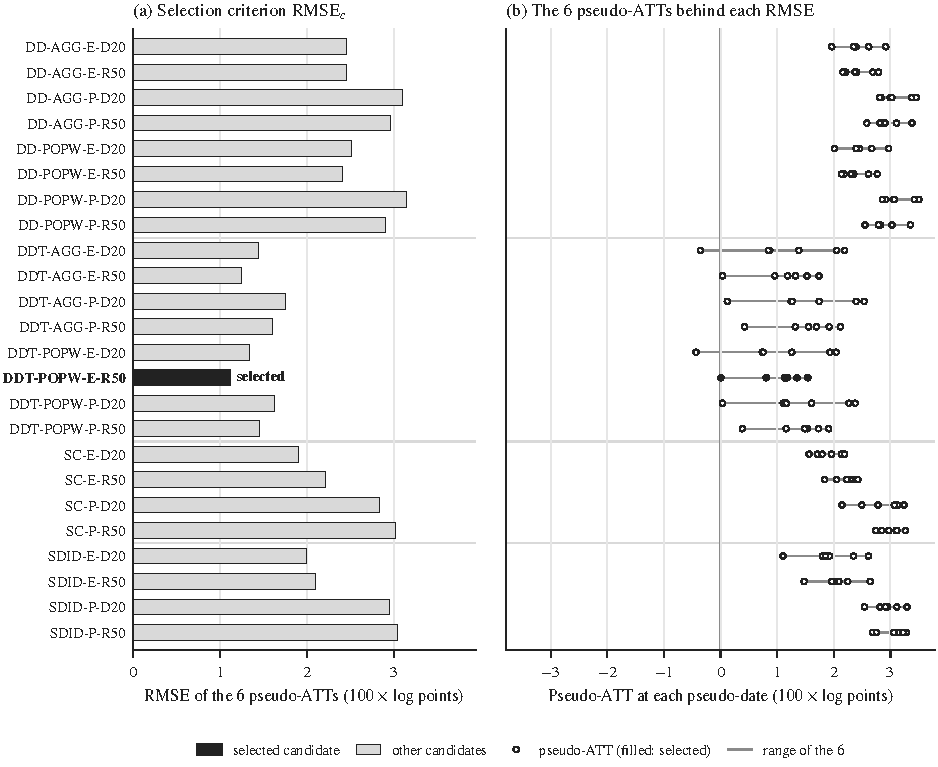
\includegraphics[width=0.88\linewidth]{figures/fig_select.pdf}
\caption{Pre-period selection of the primary estimator. Each row is one of the 24 candidates. At
each of the six pseudo-dates (2016Q1--2017Q2) California is treated as if the law had started then,
and the candidate's pseudo-ATT is its pooled estimate over the eight quarters three to ten quarters
after the pseudo-date; AB 1228 did not exist then, so a pseudo-ATT measures how far the candidate's
counterfactual misses California's path, including anything else specific to California in those
quarters, such as the rises in its general minimum wage. Panel (a): RMSE$_c$ in $100\times$ log
points (bars from zero). Panel (b): the six pseudo-ATTs behind each RMSE and their range. The
selected candidate, \cand{DDT-POPW-E-R50}, has the black bar and filled markers. The RMSEs are a
placebo criterion, not estimates with a sampling interval; the six pseudo-dates overlap, so their
pseudo-ATTs are not independent draws, and a small difference between two RMSEs is not evidence
that one estimator is better. The figure says nothing about any quarter after 2019Q4. Run
\cand{fig-select}.}
\label{fig:select}
\end{figure}

Three facts qualify the selection. First, as the design anticipated (Section~\ref{sec:select}),
the winner is a trend-adjusted candidate with the R50 pool, the kind of candidate that can track
California's own 2014--2022 general minimum-wage ramp; the rule cannot tell whether it also tracks
California's path without AB 1228 after 2023. Second, all six of the winner's employment
pseudo-ATTs are positive, from $\CaHTwoSeventeenQTwoTau$ to $\CaHTwoSixteenQTwoTau$, so most of its
RMSE is a systematic shortfall of the counterfactual, not noise. Third, the rule was applied to
employment, and H1 inherits the same estimator for wages: on log weekly wages its six pseudo-ATTs
for California are all negative, from $\CaHOneSixteenQFourTau$ to $\CaHOneSeventeenQOneTau$, so the
selected estimator fits California's pre-period wages poorly. The selected RMSE, $\SelRmse$, is
below the 2 percent bound of H2, so falsification check (i) of the identifying assumption
(Section~\ref{sec:assumption}) does not fire.

\subsection{Inference: degrees of freedom, critical values and level}
\label{sec:res-inference}

Table~\ref{tab:inference} reports, for every statistic that carries a label, the degrees of
freedom and critical values fixed by run \cand{level-mde} on data through 2019Q4, before any
post-period run. For the employment statistics of the primary (H2, H3) and of S1, the critical
values are $t$ at $\nu$: the quantiles of the decision set $L$ are less extreme. For the other-pool
check the upper ones are $t$ at $\nu$, but the lower ones, $\CritOtherPoolLoFive$ (0.05) and
$\CritOtherPoolLoTwoFive$ (0.025), come from $L$ and are more extreme than $-t_\nu$
($-\TnuOtherPoolNinetyFive$ and $-\TnuOtherPoolNinetySevenFive$), so its interval is wider on the
negative side. For H1 the quantiles of $L$ set the upper side: the upper quantiles of the 60 wage $t$ statistics in $L$,
$\LqHOneNinetyFive$ and $\LqHOneNinetySevenFive$, are far above $t_\nu$ ($\TnuHOneNinetyFive$ and
$\TnuHOneNinetySevenFive$), so they set H1's one-sided critical value and the upper end of its
interval. For S2 the SDID floor raises the upper critical values from
$\CritSTwoHiNinetyFiveNoFloor$ to $\CritSTwoHiNinetyFive$ (0.95) and from
$\CritSTwoHiNinetySevenFiveNoFloor$ to $\CritSTwoHiNinetySevenFive$ (0.975); the lower ones come
from $L$.

\begin{table}[tbp]
\centering
\caption{Degrees of freedom, critical values and level check (run \cand{level-mde}, data through 2019Q4)}
\label{tab:inference}
\small
\setlength{\tabcolsep}{3.2pt}
\begin{tabular}{@{}lrrrrrrrrrr@{}}
\toprule
& & & & & & & & \multicolumn{3}{c}{Two-sided rejection rate} \\
\cmidrule(l){9-11}
Statistic & $\nu$ & $t_{\nu,0.95}$ & $c_{\mathrm{hi}}(0.95)$ & $c_{\mathrm{hi}}(0.975)$ & $c_{\mathrm{lo}}(0.025)$ & $\mathrm{SE}_{\mathrm{pre}}$ & $k$ & all & $L$ & CA \\
\midrule
H1, wage & $\NuHOne$ & $\TnuHOneNinetyFive$ & $\CritHOneHiNinetyFive$ & $\CritHOneHiNinetySevenFive$ & $\CritHOneLoTwoFive$ & $\SePreHOne$ & $\KDiagHOne$ & $\RejHOneMaxAllTwo$ & $\RejHOneMaxSetLTwo$ & $\RejHOneMaxCATwo$ \\
H2, employment & $\NuHTwo$ & $\TnuHTwoNinetyFive$ & $\CritHTwoHiNinetyFive$ & $\CritHTwoHiNinetySevenFive$ & $\CritHTwoLoTwoFive$ & $\SePreHTwo$ & $\KDiagHTwo$ & $\RejHTwoMaxAllTwo$ & $\RejHTwoMaxSetLTwo$ & $\RejHTwoMaxCATwo$ \\
H3, year 2 $-$ year 1 & $\NuHThree$ & $\TnuHThreeNinetyFive$ & $\CritHThreeHiNinetyFive$ & $\CritHThreeHiNinetySevenFive$ & $\CritHThreeLoTwoFive$ & $\SePreHThree$ & $\KDiagHThree$ & $\RejHThreeMaxAllTwo$ & $\RejHThreeMaxSetLTwo$ & $\RejHThreeMaxCATwo$ \\
S1 & $\NuSOne$ & $\TnuSOneNinetyFive$ & $\CritSOneHiNinetyFive$ & $\CritSOneHiNinetySevenFive$ & $\CritSOneLoTwoFive$ & $\SePreSOne$ & $\KDiagSOne$ & $\RejSOneMaxAllTwo$ & $\RejSOneMaxSetLTwo$ & $\RejSOneMaxCATwo$ \\
S2 & $\NuSTwo$ & $\TnuSTwoNinetyFive$ & $\CritSTwoHiNinetyFive$ & $\CritSTwoHiNinetySevenFive$ & $\CritSTwoLoTwoFive$ & $\SePreSTwo$ & $\KDiagSTwo$ & $\RejSTwoMaxAllTwo$ & $\RejSTwoMaxSetLTwo$ & $\RejSTwoMaxCATwo$ \\
Other pool (D20) & $\NuOtherPool$ & $\TnuOtherPoolNinetyFive$ & $\CritOtherPoolHiNinetyFive$ & $\CritOtherPoolHiNinetySevenFive$ & $\CritOtherPoolLoTwoFive$ & $\SePreOtherPool$ & $\KDiagOtherPool$ & $\RejOtherPoolMaxAllTwo$ & $\RejOtherPoolMaxSetLTwo$ & $\RejOtherPoolMaxCATwo$ \\
\bottomrule
\end{tabular}

\medskip
\begin{minipage}{\linewidth}\footnotesize
\emph{Notes:} $\nu = \min(J, \hat\nu)$, the Satterthwaite degrees of freedom of $\SEn$ estimated
from the donors' pre-2020 placebo variances. $c_{\mathrm{hi}}(p)$ is the larger of $t_{\nu,p}$ and
the $p$-quantile of the 60 statistics of the decision set $L$ (the ten most populous
federal-minimum states at six pseudo-dates); $c_{\mathrm{lo}}$ likewise on the lower side; for S2
both also respect the SDID floor. $\mathrm{SE}_{\mathrm{pre}}$: root mean square of California's
standard error at the six pseudo-dates (log points). $k$: root mean square of California's six
pseudo-date $t$ statistics. Rejection rates: share of the nominal two-sided 5 percent tests that
reject with $\mathrm{SE} = \max(\SEs, \SEn)$ and $t$ at each test's own donor count, over all
pool units and California, over $L$, and over California's six tests. The binomial band around
0.05 reaches $\BandHTwoAll$ (all) and $\BandHTwoSetL$ ($L$) for the R50 statistics and
$\BandSTwoAll$ (all) for the D20 statistics. California's level is argued from the conservative
standard error, not measured: $L$ contains no state as large as California.
\end{minipage}
\end{table}

No two-sided rate over all tests or over $L$ in Table~\ref{tab:inference} is above its binomial
band. Because every donor is smaller than California, $\SEs$ is below $\SEn$ in every post-period
run, and California's standard error is $\SEn$, as the design anticipated. The one-sided rates
for California show where its own pre-period behaviour departs from the nominal level, with six
tests each: H1's lower test rejects in a share $\RejHOneMaxCALo$ of California's tests, matching
the negative wage pseudo-ATTs above, and S2's upper test in a share $\RejSTwoMaxCAUp$
(Section~\ref{sec:rob-secondary}). California's employment statistics of the primary, with
$k = \KDiagHTwo$, are small relative to their standard error, which is the conservative side.

\paragraph{Which standard error, and what the choice costs.} The H2 label depends on the
pre-specified rule $\mathrm{SE} = \max(\SEs, \SEn)$, so we report the three diagnostics the
design names for it (Section~\ref{sec:inference}). Table~\ref{tab:sechoice} gives them for the H2
statistic. First, the level check by population tercile: with the scaled $\SEs$ alone the
two-sided test rejects in a share $\RejHTwoScaledTercThreeTwo$ of the tests of the largest third
of units, the group closest to California in size, against $\RejHTwoMaxTercThreeTwo$ with the
maximum; with the unscaled $\SEn$ alone it over-rejects among the smallest third
($\RejHTwoUnscaledTercOneTwo$), where the maximum takes $\SEs$. The code-check Monte Carlo likewise
showed $\SEs$ alone over-rejecting under state-level shocks. Second, the diagnostic $k$, the root
mean square of California's own six pseudo-date $t$ statistics: $\KDiagHTwoScaled$ with $\SEs$ and
$\KDiagHTwoUnscaled$ with $\SEn$. A value of one would mean that the standard error matches
California's pre-period spread, so $\SEs$ understates that spread and $\SEn$ overstates it
severalfold; the same pattern holds for H3 ($\KDiagHThreeScaled$ against $\KDiagHThreeUnscaled$),
S1 ($\KDiagSOneScaled$ against $\KDiagSOneUnscaled$) and the other-pool check
($\KDiagOtherPoolScaled$ against $\KDiagOtherPoolUnscaled$), while for H1 ($\KDiagHOneScaled$
against $\KDiagHOneUnscaled$) and S2 ($\KDiagSTwoScaled$ against $\KDiagSTwoUnscaled$) even $\SEn$ is
close to or below California's spread. Third, Ferman and Pinto's own step, the regression of the
squared placebo estimates on a constant and $1/\mathrm{pop}_j$, which we report only as a
diagnostic: at California's six pseudo-dates its implied $\mathrm{SE}_{\mathrm{FP}}$ ranges from
$\CaHTwoSeventeenQOneFpSe$ to $\CaHTwoSixteenQOneFpSe$, against California's standard errors of
$\CaHTwoSixteenQOneSe$ to $\CaHTwoSeventeenQTwoSe$; in the real H2 run $\hat A = \HTwoFpA$ is
negative and $\hat B = \HTwoFpB$, so $\mathrm{SE}_{\mathrm{FP}} = \HTwoFpSe$: the
$A + B/\mathrm{pop}$ variance model fails here, which is not a standard error but supports not
relying on the scaled one. Read together, the diagnostics bracket California's true standard error
between $\SEs$ and $\SEn$, as the argument of Section~\ref{sec:inference} says, and show that the
maximum chosen to protect the level is far from tight for California's employment statistics. What
that costs for H2 is shown in Section~\ref{sec:res-h2}.

\begin{table}[tbp]
\centering
\caption{The H2 statistic under each standard error (run \cand{level-mde}, data through 2019Q4)}
\label{tab:sechoice}
\small
\begin{tabular}{@{}lrrrrrrr@{}}
\toprule
& \multicolumn{6}{c}{Two-sided rejection rate at nominal 5\%} & \\
\cmidrule(lr){2-7}
Standard error & Tercile 1 & Tercile 2 & Tercile 3 & All & $L$ & CA & $k$ \\
\midrule
$\SEs$ (scaled) & $\RejHTwoScaledTercOneTwo$ & $\RejHTwoScaledTercTwoTwo$ & $\RejHTwoScaledTercThreeTwo$ & $\RejHTwoScaledAllTwo$ & $\RejHTwoScaledSetLTwo$ & $\RejHTwoScaledCATwo$ & $\KDiagHTwoScaled$ \\
$\SEn$ (unscaled) & $\RejHTwoUnscaledTercOneTwo$ & $\RejHTwoUnscaledTercTwoTwo$ & $\RejHTwoUnscaledTercThreeTwo$ & $\RejHTwoUnscaledAllTwo$ & $\RejHTwoUnscaledSetLTwo$ & $\RejHTwoUnscaledCATwo$ & $\KDiagHTwoUnscaled$ \\
$\max(\SEs, \SEn)$ (pre-specified) & $\RejHTwoMaxTercOneTwo$ & $\RejHTwoMaxTercTwoTwo$ & $\RejHTwoMaxTercThreeTwo$ & $\RejHTwoMaxAllTwo$ & $\RejHTwoMaxSetLTwo$ & $\RejHTwoMaxCATwo$ & $\KDiagHTwo$ \\
\bottomrule
\end{tabular}

\medskip
\begin{minipage}{\linewidth}\footnotesize
\emph{Notes:} H2 statistic of the selected candidate (pooled log employment, R50 pool) at the six
pseudo-dates 2016Q1--2017Q2. Terciles: the pool units and California sorted by population, 1
smallest to 3 largest. $L$: the decision set; CA: California's six tests. $t$ at each test's own
donor count. $k$: root mean square of California's six pseudo-date $t$ statistics with that
standard error (one means the standard error matches California's pre-period spread).
\end{minipage}
\end{table}

Two results of the code check that preceded the design gate, echoed by run \cand{level-mde},
complete the picture. On the Proposition 99 data our exact synthetic control gives
$\PropSCsclib$ (an independent exact solve: $\PropSCexact$), and a port of the reference package's
iterative solver gives $\PropSCfwSparse$ with its default sparsification and
$\PropSCfwNoSparse$ without it, next to the printed $-19.6$ of % crew:literal
\citet[Table~1]{arkhangelsky2021synthetic}. In the Monte Carlo study, SDID with D20 donors and
pure state-level shocks rejected two-sided in a share $\McSDIDEDTwentyPureARhoZeroZeroMaxTJTwo$ of
replications at $t_J$ without autocorrelation, and $\McSDIDEDTwentyPureARhoZeroZeroFloorTwo$ with
the calibrated floor; the floor values for D20 are $\QcalDTwentyHiNinetyFive$ and
$\QcalDTwentyHiNinetySevenFive$ (upper, 0.95 and 0.975) and $\QcalDTwentyLoFive$ and
$\QcalDTwentyLoTwoFive$ (lower, 0.05 and 0.025). With unequal state-shock variances the same SDID
cell rejected in a share $\McSDIDEDTwentyHeteroARhoZeroZeroMaxTnuTwo$ even at the Monte Carlo
degrees of freedom ($\McSDIDEDTwentyHeteroARhoZeroZeroFloorTwo$ with the floor), which we report
as the size of S2's two-sided test under that design. For the selected candidate the same
unequal-variance design rejected in a share $\McDDTPOPWERFiftyHeteroARhoZeroZeroMaxTJTwo$ at
$t_J$, within its bound.

\subsection{Power, before any post-period outcome}
\label{sec:res-power}

The power quantities were computed in the same run, on data through 2019Q4, and they decided the
reach of H2 and H3 before any post-period estimate existed. The minimum detectable employment
effect at 80 percent power is $\MdeHTwo$ log points, and the half-width of the H2 90 percent
interval is $h_{90} = \HNinetyHTwo$, above the bound $b = 0.02$. The label ``no effect as large as
2\%'' (and with it ``decline smaller than 2\%'') was therefore unreachable, and the test cannot
separate the two published readings, as the design had hoped it would
(Section~\ref{sec:decision}). The probability of each label is in Table~\ref{tab:labelprob}:
``inconclusive'' had probability $\ProbTauZeroUndUndet$ with no effect and $\ProbTauAltUndUndet$
with a true decline of 3.5 percent, close to the two-year median of Clemens and coauthors. With
$t_J$ in place of $t_\nu$, which no label uses, the minimum detectable effect would be
$\MdeHTwoTJ$ and $h_{90}$ would be $\HNinetyHTwoTJ$: the degrees-of-freedom penalty is small
next to the size of the standard error. Recomputed with the real post-period standard error, the
two quantities are $\MdeHTwoPost$ and $\HNinetyHTwoPost$.

\begin{table}[tbp]
\centering
\caption{Probability of each H2 label before the post-period data were read (run \cand{level-mde})}
\label{tab:labelprob}
\small
\begin{tabularx}{\linewidth}{@{}l>{\raggedright\arraybackslash}Xrr@{}}
\toprule
Sign & Size & $\tau = 0$ & $\tau = -0.035$ \\
\midrule
negative & at least $b$: ``decline of at least 2\%'' & $\ProbTauZeroNegAtleast$ & $\ProbTauAltNegAtleast$ \\
negative & smaller than $b$: ``decline smaller than 2\%'' & $\ProbTauZeroNegSmaller$ & $\ProbTauAltNegSmaller$ \\
negative & undetermined: ``decline, size not distinguishable from 2\%'' & $\ProbTauZeroNegUndet$ & $\ProbTauAltNegUndet$ \\
undetermined & smaller than $b$: ``no effect as large as 2\%'' & $\ProbTauZeroUndSmaller$ & $\ProbTauAltUndSmaller$ \\
undetermined & at least $b$: ``inconclusive'' & $\ProbTauZeroUndAtleast$ & $\ProbTauAltUndAtleast$ \\
undetermined & undetermined: ``inconclusive'' & $\ProbTauZeroUndUndet$ & $\ProbTauAltUndUndet$ \\
positive & at least $b$: ``increase of at least 2\%'' & $\ProbTauZeroPosAtleast$ & $\ProbTauAltPosAtleast$ \\
positive & smaller than $b$: ``increase smaller than 2\%'' & $\ProbTauZeroPosSmaller$ & $\ProbTauAltPosSmaller$ \\
positive & undetermined: ``increase, size not distinguishable from 2\%'' & $\ProbTauZeroPosUndet$ & $\ProbTauAltPosUndet$ \\
\bottomrule
\end{tabularx}

\medskip
\begin{minipage}{\linewidth}\footnotesize
\emph{Notes:} From $\hat\tau = \tau + \mathrm{SE}_{\mathrm{pre}}\,T$ with $T \sim t_\nu$, the H2
critical values and $\mathrm{SE}_{\mathrm{pre}}$ of Table~\ref{tab:inference}; $\tau$ in log
points.
\end{minipage}
\end{table}

For the other two hypotheses the power run was as decisive. The minimum detectable
year-two-minus-year-one difference is $\MdeHThree$ log points, above the pre-specified threshold
of 0.04, so H3 was uninformative by rule whatever its estimate. The minimum detectable wage effect
is $\MdeHOne$, large because H1's critical value comes from the upper quantile of $L$.

\subsection{H1: weekly earnings}
\label{sec:res-h1}

The pooled 2024Q2--2026Q1 effect on California's log average weekly wage in 722513 is $\HOneAtt$
log points ($\HOnePct$ percent; about \$$\HOneDollars$ a week at the 2023Q3 level of
\$$\AwwCaBase$), with standard error $\HOneSe$ and $t = \HOneT$. The pre-specified one-sided 5
percent critical value is $\HOneCrit$, the 0.95 quantile of the decision-set wage statistics, so
the test does not reject and H1 is not supported. With $t$ at $\nu = \HOneNu$ alone the critical
value would have been $\TnuHOneNinetyFive$, and the one-sided $p$-value from $t_\nu$ is
$\HOnePUpper$, which we report for information only. The 90 percent interval is $\HOneLoNinety$
to $\HOneHiNinety$ and the 95 percent interval $\HOneLoNinetyFive$ to $\HOneHiNinetyFive$. By year,
the effect is $\HOneAttYrOne$ ($t = \HOneTYrOne$) in 2024Q2--2025Q1 and $\HOneAttYrTwo$
($t = \HOneTYrTwo$) in 2025Q2--2026Q1; the yearly tests use the pooled critical values (deviation
D5), and neither rejects. Weekly earnings per job are not the hourly wage the law sets, and nominal
wages carry differential price changes.

Three consequences follow from the design's rules. The verdict is ``not supported at the
pre-specified L-calibrated critical value'', which is not a finding that weekly earnings did not
rise. Because H1 is not supported, the employment result of H2 is reported as uninformative about
the wage floor. And the own-wage elasticities, pooled and by year, are not computed, because the
design computes them only for windows whose wage test rejects.

\paragraph{Post hoc checks of the H1 verdict (deviation D7).}
\label{sec:res-posthoc}
The results review traced the H1 critical value, and the crew then ran two report-only checks,
added after every post-period result had been seen. They come from one run, \cand{posthoc}, whose
code passed the last code review round but was changed afterwards to fix that round's minor
findings; with the human PI's agreement it was run without a further review; the ledger counts it among the analysis runs not covered by a passing
code review ($\CrewRunsUnreviewed$ in all). The two
checks point in opposite directions, and we report them only together.

The first concerns the critical value. Georgia's largest decision-set wage $t$ statistic is
$\PhGaTmax$; the other nine states' 54 tests reach at most $\PhOthersTmax$, below $t_\nu$. Georgia's published 722513 average weekly wage fell from \$$\PhGaAwwLimSvcTwoZeroOneFourQFour$
in 2014Q4 to \$$\PhGaAwwLimSvcTwoZeroOneFiveQOne$ in 2015Q1, and its year-over-year log change
less the median state's was as low as $\PhGaDevMin$ in 2015, against a largest deviation of
$\PhLargestOtherDev$ in any other state and quarter of 2015--2019; the trend windows of the 2016
pseudo-dates straddle that drop. In 2015Q1 Georgia's 722513 employment changed by
$\PhGaEmpYoyDevLimSvcTwoZeroOneFiveQOne$ relative to the median state and its 722513 establishment
count by $\PhGaEstYoyLimSvcTwoZeroOneFiveQOne$ year over year, and the weekly wages of its
full-service restaurants and of all its industries by $\PhGaAwwYoyDevFullSvcTwoZeroOneFiveQOne$
and $\PhGaAwwYoyDevTotalTwoZeroOneFiveQOne$ relative to the median; no Georgia state row of these
series is suppressed in 2014--2016. These are facts about the series; the run does not judge whether the
drop is a reporting artefact. With Georgia's own six decision-set tests removed (Georgia remaining
a donor and placebo unit), the upper decision-set quantiles fall to $\PhGaLLqNinetyFive$ and
$\PhGaLLqNinetySevenFive$, H1's critical value becomes $t_\nu = \PhGaLCritHiNinetyFive$, and the
pooled, year-one and year-two wage statistics all exceed it; the pooled 95 percent interval becomes
$\PhGaLPooledLo$ to $\PhGaLPooledHi$. Recomputing $\nu$ without Georgia's placebo variance, the
largest single share of the donors' total ($\PhGaSTwoShare$), gives $\nu = \PhNuGaOut$, a critical
value of $\PhGaLNuCritHiNinetyFive$ and a pooled interval from $\PhGaLNuPooledLo$ to
$\PhGaLNuPooledHi$. Leaving out each of the ten decision-set states in turn, only Georgia's removal
moves the critical values. But Georgia was singled out after the results were seen.

The second concerns the wage counterfactual. For the selected trend-adjusted estimator the
2022Q1--2023Q3 event-path gaps are the trend's own fit points, so the design's out-of-fit evidence
before the law is the 2014--2019 segment of the path. There the wage gap rises from
$\PhDriftWageGapStart$ in 2014Q1 to $\PhDriftWageGapEnd$ in 2019Q4, an OLS slope of
$\PhDriftWageSlope$ log points per quarter, with a root mean square of $\PhDriftWageRms$. If that
relative trend, rather than the 2022--2023 one the estimator removes, applied after 2023Q3, it
would account for
$\PhDriftWageImpliedPost$ log points at the post window's mean horizon of 6.5 quarters, against the
H1 estimate of $\HOneAtt$. But a linear extrapolation is not a test, and the 2014--2019 segment
contains California's own general minimum-wage ramp, so which relative trend applies after 2023Q3
is not identified.

Read together, the first check says that the pre-specified critical value is set by one state's
series and the second that the wage estimate may partly reflect a relative trend the estimator
does not remove. Neither changes the pre-specified verdict, and neither licenses the reading that
the first stage is established or that it is absent.

\subsection{H2: employment}
\label{sec:res-h2}

The pooled 2024Q2--2026Q1 effect on California's seasonally adjusted log employment in private
722513 is $\HTwoAtt$ log points, or $\HTwoPct$ percent. At California's mean post-window employment
of $\CaEmpPost$ that is about $\HTwoJobs$ jobs, with a 95 percent interval from $\HTwoJobsLo$ to
$\HTwoJobsHi$. The placebo standard error is $\HTwoSe$, the unscaled one ($\SEs = \HTwoSeScaled$),
and with $\nu = \HTwoNu$ the 95 percent interval is $\HTwoLoNinetyFive$ to $\HTwoHiNinetyFive$
($\HTwoPctLo$ to $\HTwoPctHi$ percent) and the 90 percent interval $\HTwoLoNinety$ to
$\HTwoHiNinety$. The 95 percent interval contains zero, so the sign is undetermined; the 90 percent
interval reaches beyond $\pm0.02$, so the size is undetermined; the label is ``inconclusive''. The
two-sided $p$-value from $t_\nu$, for information, is $\HTwoPTwo$. Figure~\ref{fig:placebo} places
California's estimate among the placebo estimates of its 50 donors.

The label rests on the pre-specified choice of the larger standard error. As a report-only note,
not the pre-specified inference: with the scaled $\SEs$ alone ($\HTwoSeScaled$, the population
scaling Dube uses) in place of $\max(\SEs, \SEn)$ and the same critical values, which for H2 are
$t$ at $\nu$, the 95 percent interval of the H2 estimate would lie entirely below zero. The design
takes the larger standard error because $\SEs$ alone over-rejects for large units in the level
check ($\RejHTwoScaledTercThreeTwo$ in the largest tercile, against $\RejHTwoMaxTercThreeTwo$ with
the maximum; Table~\ref{tab:sechoice}) and under state-level shocks in the Monte Carlo study. The
``inconclusive'' label is therefore a property of this design's conservative inference for one
treated state, not of the QCEW data alone: the width of the interval is set by the standard error
the design chose to protect the level of its tests.

The verdict run qualified the label: the placebo outcome, employment outside 722513, has a 95
percent interval that excludes zero (Section~\ref{sec:rob-placebo}), so the headline is
``inconclusive; not separable from a California-wide shock''. California's employment outside
722513 ran above its counterfactual, so a deviation shared by 722513 would bias the H2 estimate
toward zero or upward, not toward a decline; no adjustment is made, since none was pre-specified.
As H1 is not supported, H2 is also uninformative about the wage floor.

The label is the one the power run made likely before the data were read, and it is not evidence
against either published estimate: Clemens and coauthors' two-year median of about $-3.5$ percent
and Dube's near-zero estimate both lie well inside the interval, although neither is the same
estimand as ours (Section~\ref{sec:lit-estimates}).

\begin{figure}[tbp]
\centering
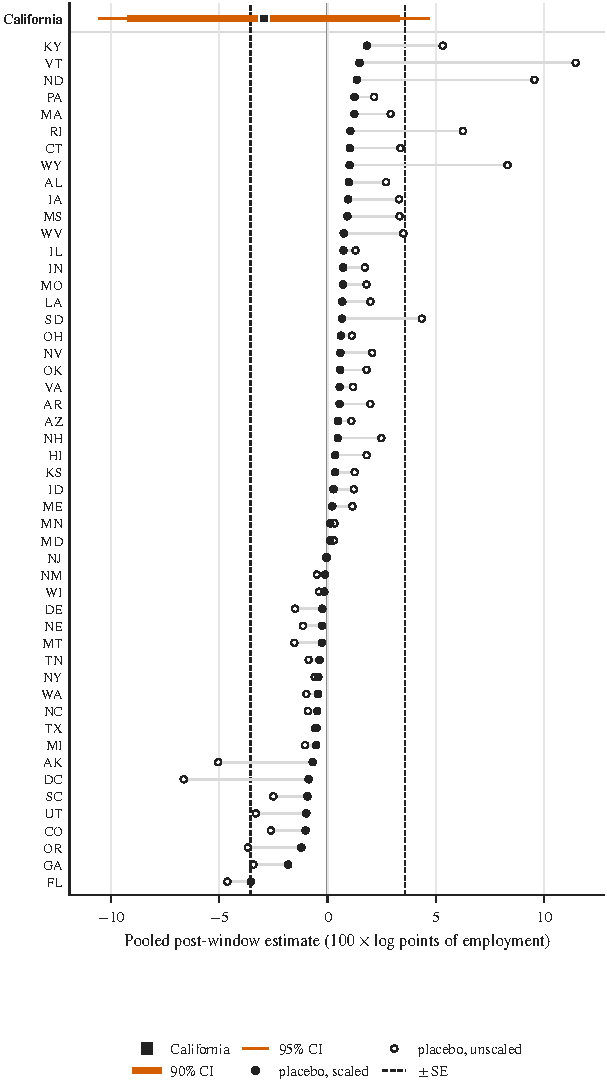
\includegraphics[width=0.52\linewidth]{figures/fig_placebo.pdf}
\caption{California's pooled H2 estimate against the placebo estimates of its 50 donors. Outcome:
seasonally adjusted log employment, NAICS 722513; estimator \cand{DDT-POPW-E-R50}; base 2023Q3, post
window 2024Q2--2026Q1; $100\times$ log points. Each donor's placebo is the same estimate with that
donor treated and the other 49 donors as its pool. Open markers: the placebo estimate; filled
markers: the same times $\sqrt{\mathrm{pop}_j/\mathrm{pop}_{\mathrm{CA}}}$. The inference uses
$\mathrm{SE} = \max(\SEs, \SEn)$, here $\SEn$; dashed lines mark $\pm\mathrm{SE}$. California's 90
percent (thick) and 95 percent (thin) intervals use the H2 critical values ($t$ at
$\nu = \HTwoNu$). The donors' placebos are not effects of any policy, the figure is not a
permutation test, and no $p$-value is read from California's rank. Run \cand{fig-placebo}.}
\label{fig:placebo}
\end{figure}

\subsection{H3: year two against year one}
\label{sec:res-h3}

The employment effect is $\HThreeYrOne$ in year one (95 percent interval $\HThreeYrOneLo$ to
$\HThreeYrOneHi$) and $\HThreeYrTwo$ in year two ($\HThreeYrTwoLo$ to $\HThreeYrTwoHi$). Their
difference is $\HThreeDiff$, with standard error $\HThreeDiffSe$ and 95 percent interval
$\HThreeDiffLo$ to $\HThreeDiffHi$. Without the power rule the H3 rule would label it ``no detectable
change''; but the minimum detectable difference is $\MdeHThree$ with the pre-period standard error
and $\MdeHThreePost$ with the real one, and the larger, $\MdeHThreeMax$, exceeds 0.04, so H3 is
``uninformative''. The yearly wage effects next to which H3 was to be read, $\HOneAttYrOne$ and
$\HOneAttYrTwo$, are not supported by their tests either, and no yearly elasticity is computed.
The data cannot say whether the effect changed as the law's premium over the general minimum fell.

% Secondary analyses, robustness and placebo checks. Every number is a macro.
% Runs: sec-cemn, sec-dube, rob-base-2023q4, rob-pre-ab257, rob-pool, rob-7225, rob-final-quarters,
% plc-nonff, plc-722511, anticip, event-path; posthoc part (c) for the employment drift (D7).
% The wage drift (r-ph-wage-*) is cited only in Section 6.4 next to the Georgia check (r-ph-h1-joint).
\section{Secondary analyses, robustness and placebo checks}
\label{sec:robustness}

Every check planned in Section~\ref{sec:robust-plan} was run once and is reported here, whatever it
shows. Table~\ref{tab:robust} collects the employment estimates. None of the checks that can
qualify the headline gives a sign category different from the primary's: all are
``inconclusive''. One check fails: the placebo outcome.

\begin{table}[tbp]
\centering
\caption{Employment estimates of the secondary analyses, robustness and placebo checks (log points)}
\label{tab:robust}
\small
\begin{tabularx}{\linewidth}{@{}>{\raggedright\arraybackslash}Xrrrl@{}}
\toprule
Specification & Estimate & 95\% interval & 90\% interval & H2-rule label \\
\midrule
Primary, \cand{DDT-POPW-E-R50} (H2) & $\HTwoAtt$ & $[\HTwoLoNinetyFive,\ \HTwoHiNinetyFive]$ & $[\HTwoLoNinety,\ \HTwoHiNinety]$ & inconclusive \\
\addlinespace
\multicolumn{5}{@{}l}{\emph{Named secondary analyses}} \\
S1, detrended DD of Clemens and coauthors, R50 aggregate & $\SOneAtt$ & $[\SOneLo,\ \SOneHi]$ & $[\SOneLoNinety,\ \SOneHiNinety]$ & inconclusive \\
S1 without the trend & $\SOneSimpleAtt$ & $[\SOneSimpleLo,\ \SOneSimpleHi]$ & & \\
S2, SDID of Dube, per capita, D20 & $\STwoAtt$ & $[\STwoLo,\ \STwoHi]$ & $[\STwoLoNinety,\ \STwoHiNinety]$ & inconclusive \\
\addlinespace
\multicolumn{5}{@{}l}{\emph{Robustness checks (selected estimator)}} \\
Base 2023Q4 (Dube's), 2024Q1 dropped & $\RobBaseFourAtt$ & $[\RobBaseFourLo,\ \RobBaseFourHi]$ & $[\RobBaseFourLoNinety,\ \RobBaseFourHiNinety]$ & inconclusive \\
Base 2022Q2, before AB 257 & $\RobPreABAtt$ & $[\RobPreABLo,\ \RobPreABHi]$ & $[\RobPreABLoNinety,\ \RobPreABHiNinety]$ & inconclusive \\
Other pool (D20) & $\RobPoolAtt$ & $[\RobPoolLo,\ \RobPoolHi]$ & $[\RobPoolLoNinety,\ \RobPoolHiNinety]$ & inconclusive \\
All restaurants (NAICS 7225), four suppressed donors dropped & $\RobAllRestaurantsAtt$ & $[\RobAllRestaurantsLo,\ \RobAllRestaurantsHi]$ & $[\RobAllRestaurantsLoNinety,\ \RobAllRestaurantsHiNinety]$ & inconclusive \\
\quad all donors, 2024Q4 dropped & $\RobAllRestaurantsAllDonorsAtt$ & $[\RobAllRestaurantsAllDonorsLo,\ \RobAllRestaurantsAllDonorsHi]$ & & \\
Final data only, 2024Q2--2025Q4 & $\RobFinalAtt$ & $[\RobFinalLo,\ \RobFinalHi]$ & $[\RobFinalLoNinety,\ \RobFinalHiNinety]$ & inconclusive \\
\addlinespace
\multicolumn{5}{@{}l}{\emph{Placebo outcomes (selected estimator)}} \\
Employment outside 722513 & $\PlcNonffAtt$ & $[\PlcNonffLo,\ \PlcNonffHi]$ & & fails \\
Full-service restaurants (722511), not a clean placebo & $\PlcFullServiceAtt$ & $[\PlcFullServiceLo,\ \PlcFullServiceHi]$ & & report only \\
\bottomrule
\end{tabularx}

\medskip
\begin{minipage}{\linewidth}\footnotesize
\emph{Notes:} Pooled 2024Q2--2026Q1 effects on seasonally adjusted log employment of California's
private NAICS 722513 (other rows as stated), base 2023Q3 unless stated. Each label is the one the
H2 rule gives, and none is the headline. S1 and S2 use their own critical values (S2 with the D20
SDID floor), the other-pool check its own, and the remaining rows the selected candidate's
employment critical values with $t$ at each run's own $\nu$. Blank cells: not reported by the run.
\end{minipage}
\end{table}

\subsection{The two published approaches}
\label{sec:rob-secondary}

\paragraph{S1, the detrended comparison of Clemens and coauthors.} Re-estimated with our 2023Q3
base, pooled post window and inference, S1 gives $\SOneAtt$ log points ($\SOnePct$ percent), with
a 95 percent interval from $\SOneLo$ to $\SOneHi$: ``inconclusive''. Their placebo rank $p$-value
is $\SOneRankP$ (one-sided). Without the trend the estimate is $\SOneSimpleAtt$ (rank
$p = \SOneSimpleRankP$). The cross-check against print reproduces their September-to-September
fixed-horizon estimates for 2023--2025 with their 48-state pool at $\CemnFhSimple$ index points
(simple) and $\CemnFhDetr$ (detrended), against $-2.74$ and $-3.72$ in
\citet[Table~3, Panel~B]{clemens2026employment}: both of ours are more negative than the printed
values, by $\CemnFhSimpleDiff$ and $\CemnFhDetrDiff$ points, a difference we have not traced.

\paragraph{S2, the SDID of Dube.} With our timing S2 gives $\STwoAtt$ log points ($\STwoPct$
percent), with a 95 percent interval from $\STwoLo$ to $\STwoHi$: ``inconclusive''. Its interval
is the narrowest of the three in Table~\ref{tab:headline}, but S2 also behaves worst for California
before the law: its six pseudo-ATTs are all positive, from $\CaSTwoSeventeenQTwoTau$ to
$\CaSTwoSixteenQTwoTau$ log points, the root mean square of California's six $t$ statistics is
$k = \KDiagSTwo$, and California's upper one-sided test rejects at a share $\RejSTwoMaxCAUp$ of
the pseudo-dates even with the maximum standard error and the SDID floor. The narrower interval is
therefore not support for a near-zero effect. S2's wage effect with the employment weights reused,
as Dube does, is $\STwoWage$ (95 percent interval $\STwoWageLo$ to $\STwoWageHi$); for the same
reason it is not an independent confirmation of the first stage. Under Dube's own timing our SDID
gives $\DubeTimingEmp$ ($100\times$ log points; scaled placebo standard error $\DubeTimingSe$),
against $-0.26$ (0.54) in \citet[Table~1, Panel~A]{dube2026labor}, a difference of
$\DubeTimingEmpDiff$, and a wage effect of $\DubeTimingWage$ against 6.99 (difference
$\DubeTimingWageDiff$). Our SDID includes an intercept and separate penalties and uses our own
seasonal factors, so this cross-check measures the combined difference from his implementation.

\subsection{Robustness checks}
\label{sec:rob-checks}

Moving the base to Dube's 2023Q4 gives $\RobBaseFourAtt$; moving it before AB 257, to 2022Q2, gives
$\RobPreABAtt$ with a wider interval; the trend is then extrapolated over a longer horizon. The other pool,
D20, gives $\RobPoolAtt$. Dropping the preliminary 2026Q1 gives $\RobFinalAtt$, so the one new
quarter moves the pooled estimate little. All four are ``inconclusive'', with point estimates
between $\RobPreABAtt$ and $\RobBaseFourAtt$, around the primary's $\HTwoAtt$.

For all restaurants (NAICS 7225) the estimate is $\RobAllRestaurantsAtt$ with the four donors
whose 2024Q4 row is suppressed dropped, and $\RobAllRestaurantsAllDonorsAtt$ with all donors and
2024Q4 dropped from the post window; both intervals contain zero. A 722513 decline with no 7225
decline was to point to reclassification or substitution toward other restaurants; neither the
722513 nor the 7225 estimate is distinguishable from zero, so the check cannot speak to it.

\subsection{Placebo outcomes}
\label{sec:rob-placebo}

Employment in all covered industries except 722513 ran above its counterfactual by
$\PlcNonffAtt$ log points ($\PlcNonffPct$ percent), with a 95 percent interval from $\PlcNonffLo$
to $\PlcNonffHi$ that excludes zero. By the pre-specified rule the H2 label is qualified as not
separable from a California-wide shock. The deviation is about as large as the H2 estimate and of
the opposite sign: if the same California-wide deviation reached 722513, the H2 estimate is biased
toward zero or upward, not toward a decline. No numerical adjustment was pre-specified and none is
made. The comparison therefore does not hold for California's aggregate labour market, which is
falsification check (iii) of the identifying assumption (Section~\ref{sec:assumption}). With two
placebo outcomes, one failure by chance alone had a probability of about 0.10; we do not discount
the failure for that.

Full-service employment (722511), reported only because covered chains are also coded there, gives
$\PlcFullServiceAtt$, with an interval from $\PlcFullServiceLo$ to $\PlcFullServiceHi$. As stated in
the plan, a null estimate here does not validate the design.

\subsection{Anticipation}
\label{sec:rob-anticip}

Between signing and the effective date (2023Q4--2024Q1), against the 2023Q3 base, the employment
effect is $\AnticipEmp$ (95 percent interval $\AnticipEmpLo$ to $\AnticipEmpHi$) and the wage
effect $\AnticipWage$ ($\AnticipWageLo$ to $\AnticipWageHi$); neither is tested. The wage interval
uses H1's decision-set critical value $c_{\mathrm{hi}}(0.975)$, so it is wide on the negative side
(Section~\ref{sec:res-inference}).

\subsection{The event path}
\label{sec:rob-event}

Figure~\ref{fig:event} shows the quarterly gap between California and the selected counterfactual.
For the trend-adjusted estimator the 2022Q1--2023Q3 gaps are residuals around the fitted trend,
so they test only curvature: their root mean square is $\EventEmpRmsGap$ for employment and
$\EventWageRmsGap$ for wages, and $\EventEmpBandsExcl$ of the seven employment and
$\EventWageBandsExcl$ of the seven wage bands exclude zero. This is not a pre-trend test. The
out-of-fit evidence before the law is the 2014--2019 segment. For employment, the gap there rises
from $\PhDriftEmpGapStart$ in 2014Q1 to $\PhDriftEmpGapEnd$ in 2019Q4, a slope of
$\PhDriftEmpSlope$ per quarter and a root mean square of $\PhDriftEmpRms$ (post hoc, deviation
D7). If that relative trend applied after 2023Q3, it would amount to about
$\PhDriftEmpImpliedPost$ log points at the post window's mean horizon, so the H2 estimate would be
biased toward zero or upward by about that amount and the counterfactual would imply a larger
decline; this is the same direction as the placebo outcome. The extrapolation is not a test, the
2014--2019 segment contains California's own general minimum-wage ramp, and the H2 label does not
change. The wage panel's out-of-fit segment bears on H1 and is reported in
Section~\ref{sec:res-posthoc}, next to the check of H1's critical value. The bands of the figure
are pointwise and use the H2 critical values in both panels, and no label is read from it; in
particular a wage band that excludes zero is not evidence against the H1 verdict.

\begin{figure}[tbp]
\centering
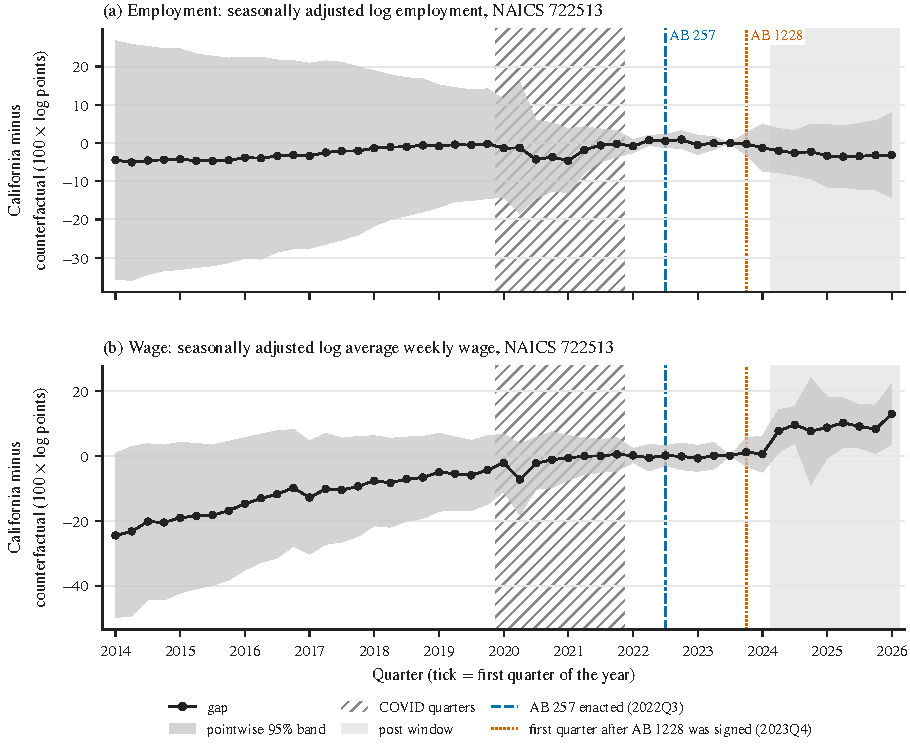
\includegraphics[width=0.85\linewidth]{figures/fig_event.pdf}
\caption{Quarterly gap between California and its estimated counterfactual, 2014Q1--2026Q1, for the
primary candidate \cand{DDT-POPW-E-R50}. Panel (a): seasonally adjusted log employment, NAICS
722513; panel (b): seasonally adjusted log average weekly wage, same estimator, weighting and pool,
with the trend fitted on the wage. Each point is California's outcome minus the counterfactual,
fitted with the base quarter 2023Q3, in $100\times$ log points. Shaded band: pointwise 95 percent
interval with $\mathrm{SE} = \max(\SEs, \SEn)$ from the donors' placebo gaps at that quarter and
the H2 critical values ($t$ at $\nu = \HTwoNu$, $c_{\mathrm{hi}}(0.975) = \CritHTwoHiNinetySevenFive$)
in both panels. H1 is decided by run \cand{h1-wage}, whose one-sided critical value
$\HOneCrit$ is far above $\CritHTwoHiNinetySevenFive$, so on the upper side the wage bands are
narrower than the H1 test. Hatched: COVID quarters, excluded from every fit. Light shading: the
post window. Dashed line: 2022Q3 (AB 257 enacted); dotted line: 2023Q4 (first quarter after AB
1228 was signed). For DDT the 2022Q1--2023Q3 gaps are residuals around the fitted trend (curvature
only); the 2014--2019 segment is outside the trend's fit. The bands are pointwise, no part of the
figure is a pre-trend test, and no hypothesis label is read from it. Run \cand{fig-event}.}
\label{fig:event}
\end{figure}

% Conclusion, limitations and deviations. Every number is a macro; process facts from process.tex.
% Deviations D1-D7: plan.json design.deviations.
\section{Conclusion}
\label{sec:conclusion}

Two years after California's \$20 fast-food minimum wage took effect, a state-level QCEW comparison
whose specification was chosen by a pre-specified rule, with inference built for one treated
state, does not determine the sign of its effect on limited-service restaurant employment. The
primary estimate is $\HTwoPct$ percent, with a 95 percent interval from $\HTwoPctLo$ to
$\HTwoPctHi$ percent; the re-estimated specifications of both published camps are also
inconclusive; and employment outside limited-service restaurants deviated from its counterfactual
by a similar amount in the opposite direction, so the estimate is not separable from a
California-wide shock. The first stage in weekly earnings is not supported at the pre-specified
critical value, and two post hoc checks of that verdict pull in opposite directions; the change
between the two years is uninformative.

The main lesson is about the cost of conservative inference with one treated state, and it was
known before the post-period data were read. With the larger of the scaled and unscaled placebo
standard errors, chosen to protect the level of California's tests, and the few effective degrees
of freedom of a placebo standard error, the 90 percent interval has a half-width of
$\HNinetyHTwo$ log points, and this design cannot tell a decline of about 3.5 percent from no
effect: ``inconclusive'' had probability $\ProbTauAltUndUndet$ under the first and
$\ProbTauZeroUndUndet$ under the second. The published estimates that disagree are both consistent
with our interval. The maximum is far from tight for California's employment statistics, and with
the scaled standard error alone the interval would lie below zero. That standard error over-rejects
if shocks have a state-level component, the threat against which the maximum was chosen a priori;
the pre-2020 diagnostics are mixed on whether such a component is present (one population tercile
supports it; the decision set, California's own tests and the Ferman--Pinto fit do not), and the
paper keeps the pre-specified maximum. Separating the published readings would need inference that is valid for California
at a smaller cost in width, more treated units, or more precise data.

\section*{Limitations and deviations from the approved design}
\label{sec:limitations}

\paragraph{Limitations.}
\begin{enumerate}
  \item \emph{Precision.} The design could not reach ``smaller than 2\%'' (Section~\ref{sec:res-power}):
        the pre-period half-width $h_{90} = \HNinetyHTwo$ exceeds $b = 0.02$, and the probability
        of ``inconclusive'' was $\ProbTauZeroUndUndet$ with no effect. The equivalence test therefore
        cannot separate the published readings, which was part of the study's motivation. The width
        is set mainly by the pre-specified maximum standard error, which overstates California's
        pre-period spread ($k = \KDiagHTwo$); with the scaled standard error alone, which
        over-rejects if shocks have a state-level component, the H2 interval would lie below zero.
        The evidence on whether that component is present is mixed
        (Sections~\ref{sec:res-inference} and~\ref{sec:res-h2}).
  \item \emph{The first stage.} H1's critical value comes from the decision-set quantile, not from
        $t_\nu$; the post hoc checks (Section~\ref{sec:res-posthoc}) show that it is set by one state
        and that the selected estimator's pre-2020 wage counterfactual drifts, and they cannot be
        resolved within this design. The selected estimator was chosen on employment and fits
        California's pre-period wages poorly. Weekly earnings per job are not hourly wages, and wages
        are nominal.
  \item \emph{Identification.} The placebo outcome fails, so a California-wide deviation cannot be
        separated from the effect. The selection rule favours candidates that track California's own
        2014--2022 minimum-wage ramp, and its winner's employment pseudo-ATTs are all positive; the
        out-of-fit 2014--2019 employment drift (post hoc) points in the same direction as the placebo
        failure. Neither is corrected for.
  \item \emph{Inference.} California's level is argued from the conservative standard error, not
        measured: no placebo state is as large. If California's own noise exceeds what its size
        implies, the tests over-reject; in the Monte Carlo design with California twice as noisy as
        its donors, the selected candidate's two-sided test at $t_J$ rejected in a share
        $\McDDTPOPWERFiftyHeteroACATwoRhoZeroZeroMaxTJTwo$ of replications. The power quantities rest
        on 2014--2019 noise; the post-period recomputations are reported next to them.
  \item \emph{Measurement.} The estimand is an intent-to-treat effect on QCEW 722513 jobs, covered
        and uncovered establishments together; covered chains are also coded in 722515 and 722511,
        and QCEW 722513 may track covered-chain employment poorly across states and over time
        \citep{melo2026covered}. The QCEW counts jobs, not hours. 2026Q1 is preliminary; the
        final-data window drops it.
  \item \emph{Unexplained cross-check differences.} Our fixed-horizon replication of Clemens and
        coauthors differs from their print by $\CemnFhSimpleDiff$ and $\CemnFhDetrDiff$ index points,
        and our SDID under Dube's timing differs from his by $\DubeTimingEmpDiff$ ($100\times$ log
        points); neither difference was traced.
  \item \emph{Not blind.} The PI and the literature scout knew the published estimates and a public
        descriptive series through March 2026 before the design was fixed
        (Section~\ref{sec:prespec}). Several rules that settle the outcomes of the code check were
        adopted after the last of the \CrewRoundsDesign{} design review rounds.
\end{enumerate}

\paragraph{Deviations from the approved design.} The first four are departures the approved design
itself makes from the track rules and the published specifications (Section~\ref{sec:departures});
the last four arose while the runs were made or the paper was written.
\begin{enumerate}
  \item[D1.] Standard errors are not clustered at the level of treatment: with one treated state,
        cluster-robust standard errors are invalid; placebo-based inference with a pre-specified
        level check is used instead.
  \item[D2.] S1 adapts the monthly fixed-horizon estimator of Clemens and coauthors to a pooled
        quarterly average, which needs seasonal adjustment; the fixed-horizon number is reported as a
        cross-check. S1 keeps their endpoint trend, whose start, 2021Q3, is the only COVID quarter
        used in any estimate.
  \item[D3.] S2 uses our implementation of Algorithm~1 of \citet{arkhangelsky2021synthetic}, with an
        intercept and separate penalties, and our seasonal factors, not Dube's code; the cross-check
        measures the combined difference.
  \item[D4.] R50 keeps Alaska and Michigan, which Clemens and coauthors drop; the cross-check against
        their print uses their 48-state pool.
  \item[D5.] The design gave no yearly H1 statistic. Recorded after the first code review and before
        any analysis run, the yearly wage tests use the pooled H1 critical values and $\nu$, so they
        are approximate. They decide whether yearly elasticities are reported; none is.
  \item[D6.] The frozen requirements pin the released \texttt{wrapt} 2.5.2 rather than the
        pre-release the design named, on the PI's instruction; no estimate depends on it.
  \item[D7.] Post hoc and report-only: run \cand{posthoc} (Section~\ref{sec:res-posthoc} and the
        employment drift in Section~\ref{sec:rob-event}) was added after the results review had
        seen every post-period result. Its code passed the last of the \CrewRoundsCode{} code review
        rounds; that round's minor findings were then fixed and, with the human PI's agreement, the
        run was made without a further review, so no code review covered the code it ran; the second
        results-review round read that code, the same file that ran, after the run. The ledger counts it among
        the analysis runs not covered by a passing code review ($\CrewRunsUnreviewed$ in all). It reports facts
        about Georgia's 2014--2015 series, the H1 critical values without Georgia's decision-set tests
        and with $\nu$ recomputed, a leave-one-out over the ten decision-set states, and the
        2014--2019 drift of the event path. It changes no label. Known defect: its leave-one-out
        change flags (\texttt{b\_loo\_*\_changes\_chi}, \texttt{b\_loo\_n\_changing},
        \texttt{b\_loo\_changing\_states} and the matching line of its log) all read 1, because they
        compare values stored at ten significant digits with a tolerance of $10^{-12}$; no claim uses
        them, the statement that only Georgia moves the critical value rests on the critical values
        themselves, and a clean rerun reproduces the same flags.
  \item[D8.] Descriptive and report-only: run \cand{describe}, added at the paper stage after the
        paper review asked for a summary-statistics table, produces only the levels of
        Table~\ref{tab:sumstats} (means of employment, average weekly wage and establishments for
        California and the two pools, and sample sizes) and no statistic comparing California with
        another unit or one period with another. The code review rounds had been used, so it was
        run without a code review, with the human PI's agreement; the ledger counts it among the
        analysis runs not covered by a passing code review. It feeds the table only and changes no
        label.
\end{enumerate}

\paragraph{How the results were checked.} The results were reviewed in \CrewRoundsResults{} rounds
by a reviewer agent that did not produce them, before the human PI approved them. The ledger holds
\CrewRuns{} runs (\CrewRunsAnalysis{} analysis runs); \CrewRunsSuperseded{} were replaced by a later
run with the same identifier and are archived. Clean rerun of every run from scratch, as recorded
when this version was compiled: \CrewRerunStatus{}, with \CrewRerunReproduced{} of
\CrewRerunTotal{} runs reproduced.


\section*{AI-use statement}

This paper was drafted by a crew of AI research-assistant agents
(Free-Research-Crew, protocol v0.2) under the direction of the human author, Bryce Wang.
He chose the topic from a proposal and approved the research question (2026-11-21, 05:35
UTC), the design (2026-11-21, 11:41 UTC) and the results (2026-11-21, 14:12 UTC), each in
chat after reading the Reviewer's verdict. The manuscript itself is subject to the
submission gate. He takes responsibility for the paper's content.

% Counts are macros from process.tex (`crew.py numbers`); who did what is taken from
% log.jsonl, reviews/ and briefs/.
\begin{itemize}
  \item \textbf{Roles and models.} Every role (PI, Scout, Designer, Data RA, Econometrician,
        Figures RA, Writer, Reviewer and Replicator) ran on Claude Opus 5.5
        (\texttt{claude-opus-5-5}) in Claude Code, each role as a separate agent. The PI
        proposed the topic, drafted the question and hypotheses, wrote the contribution
        statement, recorded deviations D5--D8 and corrected threat T14 after the results
        gate; the Scout found and verified the sources; the Designer wrote the design and
        deviations D1--D4; the Data RA fetched and prepared the data; the Econometrician
        wrote and tested the estimation code, executed the analysis runs, including the
        post hoc and descriptive runs, and wrote the result claims; the Figures RA wrote the figure scripts
        and drew the figures; the Writer drafted this paper from the claims; the Replicator
        ran the clean rerun. The PI's brief to each role is archived in \texttt{briefs/}.
  \item \textbf{Review.} The Reviewer ran \CrewReviewRounds{} rounds on
        \CrewReviewerModels{} (\CrewReviewIndependence{}: a new context in every round, the
        same model family as the other roles): \CrewRoundsQuestion{} on the question,
        \CrewRoundsLiterature{} on the literature, \CrewRoundsDesign{} on the design,
        \CrewRoundsCode{} on the code, \CrewRoundsResults{} on the results and
        \CrewRoundsPaper{} on the paper. It raised \CrewFindingsCritical{} critical,
        \CrewFindingsMajor{} major and \CrewFindingsMinor{} minor distinct findings (a
        finding carried into a later round is counted once, at its latest severity). The
        last round of each completed stage passed. Four sets of changes were made after
        the last round of their stage and reached the human at the next gate without
        another round of that stage: the design's responses to the check-methods failures
        (the SDID critical-value floor, the two-part synthetic-control check and the
        adopted implementation choices), which the code review then checked against the
        code; two report-only additions to the design (findings D14 and D15); claim-text corrections after the third results round (findings R12 and R13); and
        the PI's correction of threat T14 after the results gate (the 2025 quarters are final), which changes no analysis.
  \item \textbf{Runs.} \CrewRuns{} runs in the ledger (\CrewRunsAnalysis{} analysis,
        \CrewRunsDataPrep{} data preparation); \CrewRunsSuperseded{} were replaced by a
        later run with the same id and archived (the first data fetch, replaced to drop two metrics that a clean rerun could not reproduce, and the
        first run of the method checks, whose failures led to the design changes described above; no run behind
        a result claim was replaced); \CrewRunsUnreviewed{} analysis runs were not covered
        by a passing code review, both after the fourth and last code-review round and both
        with the human author's consent in chat: the post hoc run (deviation D7), whose
        code was changed to add the leave-one-out check the Reviewer asked for, and the
        descriptive run behind the summary-statistics table (deviation D8), added at the
        paper stage; the paper review read both runs' outputs.
  \item \textbf{Replication.} The Replicator's clean rerun (\texttt{crew.py rerun}, in a
        fresh environment built from \texttt{code/requirements.txt}) has status
        \CrewRerunStatus{}: \CrewRerunReproduced{} of \CrewRerunTotal{} runs reproduced.
        Whether the work can be rerun from scratch is what this record states, not
        something the authoring roles assert.
  \item \textbf{Not blind.} The PI and the Scout knew the published estimates and a
        published descriptive index of California fast-food employment and weekly wages
        through 2026Q1 before the design was fixed; the primary specification was
        therefore chosen by a rule on data through 2019, and the analysing roles computed
        nothing on post-2023Q3 outcomes before the design gate.
  \item \textbf{Findings accepted over the Reviewer's objection.} None.
  \item \textbf{Evidence.} Every result number in the text, the tables and the figure
        captions is a macro generated from the metrics of a logged run. The numbers typed
        by hand are design facts fixed before any analysis run, published numbers quoted
        from the literature as the Scout's source notes record them, and process facts
        such as dates. The full workspace, including every brief, review and run record, is
        published with the paper.
\end{itemize}


\bibliographystyle{plainnat-keepcase}
\bibliography{../refs}

\end{document}
